%\documentclass[prl,12pt,onecolumn,nofootinbib,notitlepage,english,superscriptaddress]{revtex4-1}
\documentclass[utf8,latin9]{frontiersFPHY} 
%\usepackage[latin9]{inputenc}

\usepackage{url,lineno,microtype,subcaption}
\usepackage[onehalfspacing]{setspace}
\renewcommand{\rmdefault}{cmr}
%\usepackage[T1]{fontenc}
\setcounter{secnumdepth}{2}
\setcounter{tocdepth}{2}
\usepackage{color}
%\usepackage{babel}
\usepackage{latexsym}
\usepackage{float}
\usepackage{amsmath}
\usepackage{amsfonts}
\usepackage{amsthm}
\usepackage{graphicx}
%\usepackage{times}   %% Times Roman font
\usepackage{esint}
%\usepackage{subfigure}
\usepackage{verbatim}
\usepackage{braket}
\usepackage{footmisc}
\usepackage{tikz}
\usetikzlibrary{shapes,arrows,calc}

\usepackage[unicode=true,pdfusetitle,
 bookmarks=false,colorlinks=true,citecolor=blue,urlcolor=blue,linkcolor=red]{hyperref}
%\makeatletter
%%%%%%%%%%%%%%%%%%%%%%%%%%%%%% LyX specific LaTeX commands.
%\special{papersize=\the\paperwidth,\the\paperheight}

%%%%%%%%%%%%%%%%%%%%%%%%%%%%%% Textclass specific LaTeX commands.
%\@ifundefined{textcolor}{}
%

%\@ifundefined{date}{}{\date{}}
%\AtBeginDocument{
  \def\labelitemi{\(\rhd\)}
%}
\makeatother

%\setlength{\belowcaptionskip}{-7pt}
\newcommand{\SAVE}[1]{}
\newcommand{\HJC}[1]{{\color{RED}{\bf HJC: #1}}}
\newcommand{\BDB}[1]{{\color{RED}{\bf BDB: #1}}}
\newcommand{\HHZ}[1]{{\color{GREEN}{\bf HHZ: #1}}}
\newcommand{\lucas}[1]{{\color{BLUE}{\bf LKW: #1}}}

\newcommand{\prlsec}[1]{\emph{#1---}}
\newcommand{\Ncal}{{\mathcal N}}
\newcommand{\T}{{\mathbf{T}}}
\newcommand{\Jbq}{{J_{bq}}}
\newcommand{\DK}[1]{{\color{BLUE}{\bf DK: #1}}}


%%added for sub figures
\newcommand{\subfigimg}[3][,]{%
  \setbox1=\hbox{\includegraphics[#1]{#3}}% Store image in box
  \leavevmode\rlap{\usebox1}% Print image
  \rlap{\hspace*{33.5pt}\vspace*{12pt}\raisebox{\dimexpr\ht1-0.95\baselineskip}{#2}}% Print label
  \phantom{\usebox1}
}

\renewcommand{\thefootnote}{\fnsymbol{footnote}}
\renewcommand\abstractname{}
%\title{From real materials to model lattice Hamiltonians: multi-scale modelling of strongly correlated electronic systems 
 %      with information from many body wavefunctions}
%\title{From real materials to model lattice Hamiltonians using \textit{ab-initio} density matrix downfolding}
%\linenumbers

\def\keyFont{\fontsize{8}{11}\helveticabold }
\def\firstAuthorLast{H. Zheng et al.} %use et al only if is more than 1 author
\def\Authors{Huihuo Zheng\,$^{1}$, Hitesh J. Changlani\,$^{2}$, Kiel Williams\,$^{3}$, Brian Busemeyer\,$^{3}$, and Lucas K. Wagner\,$^{*3}$}
% Affiliations should be keyed to the author's name with superscript numbers and be listed as follows: Laboratory, Institute, Department, Organization, City, State abbreviation (USA, Canada, Australia), and Country (without detailed address information such as city zip codes or street names).
% If one of the authors has a change of address, list the new address below the correspondence details using a superscript symbol and use the same symbol to indicate the author in the author list.
\def\Address{$^{1}$Argonne Leadership Computing Facility, Argonne National Laboratory, 9700 South Cass Avenue, Lemont, 60439, Illinois, USA\\
$^{2}$Department of Physics and Astronomy, Johns Hopkins University, Baltimore, Maryland 21218, USA \\
$^{3}$Department of Physics and Institute for Condensed Matter Theory, University of Illinois at Urbana-Champaign, 
1110 West Green St, Urbana IL 61801, USA }
% The Corresponding Author should be marked with an asterisk
% Provide the exact contact address (this time including street name and city zip code) and email of the corresponding author
\def\corrAuthor{Lucas K. Wagner}

\def\corrEmail{lkwagner@illinois.edu}

\begin{document}
\onecolumn
\firstpage{1}

%\renewcommand\abstractname{}
%\title[Multi-scale modelling]{From real materials to model lattice Hamiltonians: multi-scale modelling of strongly correlated electronic systems 
%       with information from many body wavefunctions}
\title[Density matrix downfolding]{From real materials to model lattice Hamiltonians with density matrix downfolding}
\author[\firstAuthorLast ]{\Authors} %This field will be automatically populated
\address{} %This field will be automatically populated
\correspondance{} %This field will be automatically populated
\extraAuth{}
\maketitle
%\author{Hitesh J. Changlani}
%\affiliation{Department of Physics and Astronomy, Johns Hopkins University, Baltimore, Maryland 21218, USA}
%\author{Huihuo Zheng}
%\affiliation{
%Argonne Leadership Computing Facility, Argonne National Laboratory, 9700 South Cass Avenue, Lemont, 60439, Illinois, USA}
%\author{Kiel Williams}
%\affiliation{Department of Physics and Institute for Condensed Matter Theory, University of Illinois at Urbana-Champaign, 
%1110 West Green St, Urbana IL 61801, USA}
%\author{Brian Busemeyer}
%\affiliation{Department of Physics and Institute for Condensed Matter Theory, University of Illinois at Urbana-Champaign, 
%1110 West Green St, Urbana IL 61801, USA}
%\author{Lucas K. Wagner}
%\affiliation{Department of Physics and Institute for Condensed Matter Theory, University of Illinois at Urbana-Champaign, 
%1110 West Green St, Urbana IL 61801, USA}
%\date{\today}
%\maketitle

%\textbf{
\begin{abstract}
Given a realistic quantum material with all its intrinsic complications, how does one develop a 
simple reliable model for understanding its properties? Theoretical insight has been the key driver of 
this process leading to simple few-band pictures. When the interactions are comparable 
to or much stronger than the kinetic energy, it is convenient to adopt the real space lattice 
approach and work with Hubbard or Kanamori type Hamiltonians involving only the low energy electrons. 
But this is not an easy task, since the effective Hamiltonian involves a considerable renormalization of parameters with respect 
to the bare Coulomb values. While the kinetic energy is dominated by contributions from bands or states energetically 
near the Fermi level, screened interactions depend on states even \emph{far} away from it, leading to Hubbard U's 
that have been traditionally hard to reliably determine. 
Here we discuss an approach that treats the kinetic and potential parts of the Hamiltonian 
democratically, avoids "double counting", 
and one that provides a transparent way of obtaining effective Hamiltonians using data from many body wavefunctions, 
and whose validity can be systematically checked.
We emphasize that determining the effective Hamiltonian reliably is crucial for 
several applications in physics and chemistry not only for quantitative accuracy, but also a 
correct qualitative picture of strongly correlated materials. 
\tiny
 \keyFont{ \section{Keywords:} downfolding, effective model, strongly correlated system} %All article types: you may provide up to 8 keywords; at least 5 are mandatory.
\end{abstract}
%}
\section{Introduction to downfolding the many electron problem}

One of the most sought-after, yet often daunting, endeavors for physicists is to develop 
an intuitive understanding of physical phenomena involving intrinsically complicated materials 
using simplified models. These models are expected to capture the essence of the physics, and are formulated in terms 
of the most relevant physical degrees of freedom related to the observed phenomena. 
For example, at high temperature and low density when quantum effects are relatively insignificant, the ideal gas model 
successfully captures the statistical properties of $10^{23}$ H$_{2}$ molecules in a box, 
without any detailed knowledge of the fundamental constituent of H$_{2}$. This approach is valid when we are interested in 
phenomena at certain energy scale (or length scale), while the degrees of freedom at other length scales which are not 
dynamically excited simply renormalize the dynamics of the low energy degrees of freedom. 

This principle, the basis of the renormalization group~\cite{Wilson}, 
has also been widely employed in condensed matter physics. In the past few decades, several studies 
have been dedicated to describing complex systems (for example, the high $T_c$ cuprates and other transition metal oxides), those of 
primary interest here are strongly correlated systems. These are systems where the effects of Coulomb 
interactions are comparable to or more important than the kinetic energy and the picture of 
localized rather than itinerant electrons is more pertinent. This has motivated an approach beyond the 
traditional band theory approach, involving model Hamiltonians such as the Hubbard~\cite{Hubbard}, t-J~\cite{tJSpalek} 
and Heisenberg models, defined only in terms of the valence electrons. 
While these models have been extensively studied analytically and numerically, and have significantly 
enhanced our understanding of strongly correlated physics, their effectiveness 
for describing a real complex system of interest is often unclear. 
%In addition, efforts to obtain the optimal parameter values still remains very much an active area of research, often requiring experimental inputs. 
%This is compounded by the fact that all the parameters are not independent of each other and 
%the value of one heavily influences the value of the other. The presence of multiple competing energy scales of similar strength 
%is, in fact, the source of rich phase diagrams that 
%emerge under a variety of conditions - doping, pressure, 
%temperature, all heavily dependent on material-specific properties. 
This motivates the need to determine reliable low energy effective Hamiltonians that can capture all the necessary details, while 
remaining simple enough to be simulated accurately.  

\begin{figure}[htpb]
\centering
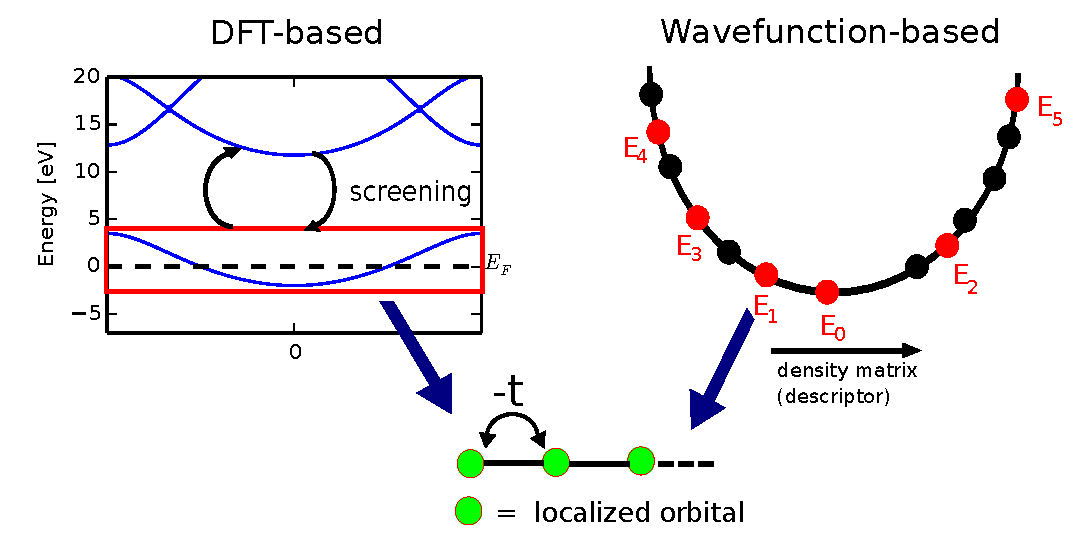
\includegraphics[width=1\linewidth]{./Figures/figure1.eps}
\caption{Schematics for downfolding a simple ab-initio system (here the hydrogen chain) 
in DFT based methods (left) and the wavefunction based AIDMD (right). Localized one particle functions 
are constructed in both methods and serve as the one body space for the model Hamiltonian. The DFT based methods 
use Kohn Sham orbitals and screening models to estimate the interactions. AIDMD uses a database of low energy 
all electron many-body wavefunctions ($\psi_i$). This "low energy basin" 
(shown abstractly in the space of descriptors) need not consist of exact eigenstates ($E_i$).}
\label{fig:lowenergybasin_schematic}
\end{figure}	


%In complex systems such as high $T_c$ cuprates, it is unclear to what extent can these models describe the reality \cite{Anderson2013}. 
%Since strongly correlated systems are  the macroscopic phenomena are strongly dependent on material-specific properties, motivating the need to determine the effective Hamiltonians that can capture all necessary details. 
%In strongly correlated systems, the macroscopic phenomena are strongly dependent on material-specific properties, motivating the need to determine the effective Hamiltonians that can capture all necessary details. 
%\HJC{Downfolding: How should we connect our intuitive understanding of coarse graining with condensed matter concepts}
%The reliable simulation of strongly correlated systems remains a major challenge in physics, chemistry, and materials science. 
%On the other hand are approximate model Hamiltonians (such as the Hubbard model) 
%which describe the low energy physics solely in terms of the valence electrons and 
%are crucial to our understanding of physical phenomena such 
%as antiferromagnetism and high temperature superconductivity. 
%However, transitioning from actual materials to an effective Hamiltonian on a lattice relies 
%on physical insight and/or fits to experimental data, and this notion is not always rigorously well justified.

The endeavor we pursue here is to develop a multi-scale approach in which the effective interactions between 
quasiparticles (such as dressed electrons) are determined after an \textit{ab-initio} simulation (but not necessarily exact 
solution) of the continuum Schroedinger equation involving all the electrons. This reduction 
of the Hilbert space is known as ``downfolding". The resultant "lattice model" can be efficiently and accurately 
solved for large system sizes using techniques designed and suited for small local Hilbert spaces- these include 
exact or selected diagonalization~\cite{DeRaedt,Tubman_selci,Holmes_Tubman_Umrigar}, density matrix renormalization group 
(DMRG)~\cite{White1992}, tensor networks~\cite{PEPS,Changlani_CPS,NeuscammanCPS}, 
dynamical field theory (DMFT)~\cite{}, density matrix embedding (DMET)~\cite{DMET_2012} and 
lattice quantum Monte Carlo (QMC) methods~\cite{Scalapino, Trivedi_Ceperley, Zhang_AFQMC, Sandvik_loops, Prokofiev, 
Booth2009,SQMC,Holmes_Changlani_Umrigar, Booth2013}. These methods have also been used to obtain 
excited states and dynamical correlation functions, that have been difficult in \textit{ab-initio} approaches. 
%Full \textit{ab-initio} wavefunction based calculations are computationally infeasible for large system sizes. 
In addition to being computationally expensive, \textit{ab-initio} approaches lack the accuracy to resolve 
low energy scales. They do, however, yield the correct low energy basin in which the effective description of the problem lives, 
schematically represented in Fig.~\ref{fig:lowenergybasin_schematic}.

Downfolding has most commonly been carried out using approaches based on density functional theory (DFT). 
The kinetic part is obtained from a standard 
DFT calculation which is projected onto localized Wannier functions and 
gives an estimate of the effective hoppings of the lattice model~\cite{Pavirini}. 
Then, to estimate the interactions, one assumes a model of screening of the Coulomb interactions 
(based on RPA, for example) which is determined from the knowledge of the single particle (Kohn Sham) 
DFT orbitals. Since effects of interactions between the orbitals (one body space) of interest, have already 
been accounted for by DFT, a "double counting correction" is required to obtain the final 
downfolded Hamiltonian. The approach has been developed and widely applied~\cite{}; 
but remains an active area of research~\cite{Haule_doublecounting}, due to 
absence of internal checks on the approximation. 
%a clear shortcoming is the absence of a systematic way of checking 
%the internal accuracy of the approximation. Improving double counting estimates remains an active area of 
%research~\cite{Haule_doublecounting}.

There are other downfolding approaches that include the traditional Lowdin method, coupled to a stochastic 
approach~\cite{Tenno,Zhou_Ceperley} and the related method of canonical transformations~\cite{White_CT, Yanai_CT}. 
These share the same aims as us, in the sense that they work with 
in a many body setting and involve working with wavefunctions. 

Our primary focus is to downfold based on results of \textit{ab initio} wavefunctions, involving all electrons, 
these explicitly provide access to properties encoded compactly in the form of reduced 
density matrices (RDMs) or correlation functions. Crucially, we do not commit ourselves to 
knowledge of exact eigenstates (a challenging endeavor) - rather we "learn" the effective Hamiltonian from a 
intelligently constructed database of low energy wavefunctions and their associated expectation values. 
Our aim is thus to discuss the development and application of a new set of methods, christened 
"ab-initio density matrix downfolding" (AIDMD)~\cite{Changlani2015},which by nature of their formulation, 
restore the democracy between kinetic and potential part of the Hamiltonian. There is no double counting involved and it is straightforward 
to judge the accuracy of the effective Hamiltonian. While our prescription applies to any wavefunction based method, 
we have primarily chosen to work with the \textit{ab-initio} QMC approach~\cite{Ceperley_Alder,Foulkes_review}. 
The QMC method works directly in the real space continuum and explicitly introduces correlations (via Jastrow factors) 
into trial wavefunctions of non-interacting electrons (Slater determinants). 
The details of the method, relevant for AIDMD, will be clarified at appropriate points 
in the text. More QMC related specifics are described in our earlier work~\cite{Changlani2015,}, but will not be 
reiterated here to focus solely on the downfolding aspect of the work. 

%What sort of accuracy should one expect with effective Hamiltonians and AIDMD? The holy grail of quantum chemistry 
%and electronic structure is to obtain an energy of 1 mHa (0.027 eV) per atom which remains an open challenge
%despite decades of work. The effective Hamiltonian approach largely ameliorates this problem,  only 
%relative energies (excitation spectrum) are important, neither the total energy (nor its accuracy) is of particularly 
%fundamental interest. This, of course, is contingent on the cancellation of the large energy associated with the core electrons, 
%whose role is primarily in renormalizing the effective interactions of the active (valence) electrons.
%Our previous experience suggests spectra can be accurately determined to 0.2 eV (or less)~\cite{Changlani2015} 
%and systematically improved with more data and more refined effective Hamiltonians.  In our view the main advantage is that 
%the effective Hamiltonian opens up many avenues for quantities not easily calculated in ground state approaches - namely excitation spectra 
%and finite temperature properties. On a conceptual level, AIDMD reveals the types of terms are important (and how much), 
%what is missing and how it could be rectified. It is also possibly best suited for extended systems (solids) where 
%there is often a clear separation of energy scales associated with the 
%core, active (valence) and virtual electronic spaces. Finally we would like to textitasize that AIDMD, though conceptually simple, 
%is still a method in its development stages, with room for several algorithmic improvements. 

The paper is organized as follows. In Section 2, we clarify and make precise what it means to downfold 
a many-electron problem to a few-electron problem. We recast the problem into minimization 
of a cost function that needs to be optimized to connect the many and few body problems. We further 
these notions both in terms of physical as well as information science descriptions, which allows us to connect to 
compression algorithms in the machine learning literature. 
Section 3 discusses several representative examples where we consider multiband lattice models 
and ab-initio systems to downfold to a simpler lattice model. 
%Section 3a gives a concrete example of downfolding from 
%the three band model (relevant to the cuprates) to the one band model - the map between the bare and 
%effective particles and parameters will be explicitly elucidated here. These concepts are directly applied 
%to a simple yet non-trivial \textit{ab-initio} problem - the hydrogen chain in section 3b where we are able to 
%systematically quantify several aspects of the effective Hubbard model describing it. Section 3c 
%shows a more advanced application to graphene. We focus on the renormalization and screening effects that arise 
%due to the presence of core (sigma) electrons, a comparison to its hydrogen counterpart on the honeycomb lattice 
%clearly elucidates why graphene is a semimetal not an insulator in vacuum. 
Finally, in Section 4, we discuss future prospects of applications of the AIDMD method, ongoing challenges 
and clear avenues for methodological improvements. 



\newtheorem{theorem}{Theorem}
\newtheorem{definition}{Definition}
\newtheorem{lemma}{Lemma}


\section{Downfolding as a compression of the energy functional}
\label{sec:theory}
\subsection{Theory} 
In this section, we will develop a sufficient criterion for an effective Hamiltonian $H_{eff}$ to reproduce the spectrum of a first-principles Hamiltonian $H$ within a chosen low-energy space. 
The criterion is that if a wave function $\ket{\Psi}$ is drawn from the low-energy space, then the expectation values of the effective and first principles Hamiltonian must match for that wave function.
We then use the concept of \textit{descriptors} to help parameterize the effective Hamiltonian in terms of expectation values on wave functions sampled from the low-energy space, such as hopping and two-body interaction terms
\subsubsection{Energy functional}
Suppose we start with a quantum system with Hamiltonian $H$ and Hilbert space ${\mathcal H}$.

\begin{definition}
Let the energy functional be $E[\Psi] = \frac{\bra{\Psi}H\ket{\Psi}}{\braket{\Psi|\Psi}}$ for a wavefunction $\ket{\Psi} \in {\mathcal H}$.
\end{definition}


\begin{theorem}
\label{theorem:criticalpoint}
$E[\Psi]$ has a critical point only where $\Psi$ is an eigenstate of $H$.
\end{theorem}
\begin{proof}
\begin{eqnarray}
\frac{\delta }{\delta \Psi^*}  E[\Psi] = \frac{\delta}{\delta \Psi^*}\frac{\langle \Psi |H|\Psi\rangle}{\langle \Psi |\Psi\rangle} = \frac{H|\Psi\rangle}{\langle \Psi |\Psi\rangle} - \langle \Psi |H|\Psi\rangle \frac{|\Psi \rangle}{|\langle \Psi | \Psi\rangle|^2} =\frac{ (H-E[\Psi])|\Psi\rangle }{\langle\Psi|\Psi\rangle}\,.
\end{eqnarray}
Therefore, 
$\frac{\delta }{\delta \Psi^*}  E[\Psi] = 0$ if and only if $(H-E[\Psi])|\Psi\rangle =0$, i.e., $\Psi$ is an eigenvector of $H$ corresponding to eigenvalue $E[\Psi]$.  
\end{proof}

\subsubsection{Low energy space} 

\begin{definition}
Let $\mathcal{LE}(H,N)$ be a subset of ${\mathcal H}$ spanned by $N$ vectors given by the lowest energy solutions to $H\ket{\Psi_i}=E_i{\Psi_i}$. 
\end{definition}

\begin{definition}
$H_{eff}$ is an operator on the Hilbert space ${\mathcal {LE}(H,N)}$.	 
\end{definition}

\begin{definition}
The effective model $E_{eff}[\Psi]=\frac{\bra{\Psi}H_{eff}\ket{\Psi}}{\braket{\Psi|\Psi}}$ is a functional from $\mathcal{LE} \rightarrow \mathbb{R}$. 
\end{definition}

If $\ket{\Psi}\in \mathcal{LE}$ and $\ket{\Phi}\in {\mathcal H} \setminus \mathcal{LE}$, then $\ket{\Psi} \oplus \ket{\Phi} \in {\mathcal H}$.
In the following, we will use the direct sum operator $\oplus 0$ to translate between the larger ${\mathcal H}$ and the smaller $\mathcal{LE}$. 

\begin{lemma}
\label{lemma:zeroderiv}
Suppose that $\ket{\Psi}\in \mathcal{LE}$ and $\ket{\Phi} \in {\mathcal H} \setminus \mathcal{LE}$. 
Then $\left.\frac{\delta E[\Psi \oplus \Phi]}{\delta \Phi}\right|_{\Phi=0}=0$. 
\end{lemma}
\begin{proof}
$\langle \Psi\oplus 0 | H | 0\oplus \Phi \rangle=0$ because the two states have non-overlapping expansions in the eigenstates of $H$. 
Using that fact, we can evaluate
\begin{align}
\left.\frac{\delta E[\Psi \oplus \Phi]}{\delta \Phi}\right|_{\Phi=0} &= \left.\frac{\left(H-E[\Psi\oplus\Phi]\right) \ket{\Phi} }{\braket{\Psi|\Psi} + \braket{\Phi|\Phi}} \right|_{\Phi=0} = 0.
\end{align}
\end{proof}
This is equivalent to noting that $H$ is block diagonal in the partitioning of ${\mathcal H}$ into $\mathcal{LE}$ and ${\mathcal H} \setminus \mathcal{LE}$.
Importantly, if $\ket{\Psi} \in \mathcal{LE}$, then $\frac{\delta  E[\Psi\oplus 0] }{\delta (\Psi\oplus 0)^*} = \ket{\Psi'} \oplus 0$, where $\ket{\Psi'} \in \mathcal{LE} $. 

\begin{theorem}
\label{theorem:matching}
Assume $ E[\Psi\oplus 0]  = E_{eff}[\Psi]+C$ for any $\ket{\Psi } \in \mathcal{LE}$, where $C$ is a constant. 
Then $(H_{eff}+C)|\Psi\rangle\oplus 0 = H (|\Psi\rangle \oplus 0)$.
\end{theorem}
\begin{proof}
Note that
\begin{align}
	\frac{\delta E[\Psi\oplus 0]}{\delta (\Psi\oplus 0)^*}=\frac{(H-E[\Psi\oplus 0])\ket{\Psi\oplus 0} }{\braket{\Psi|\Psi}}
	\label{eqn:psider}
\end{align}
and 
\begin{align}
	\frac{\delta E_{eff}[\Psi]}{\delta \Psi^*}=\frac{(H_{eff}-E_{eff}[\Psi])\ket{\Psi} }{\braket{\Psi|\Psi}}.
	\label{eqn:psieffder}
\end{align}
Since the derivatives are equal, setting Eq.~\eqref{eqn:psider} equal to Eq.~\eqref{eqn:psieffder},
\begin{align}
	 H\ket{\Psi\oplus 0}= (H_{eff}+E[\Psi\oplus 0]-E_{eff}[\Psi])\ket{\Psi}\oplus 0 =(H_{eff}+C)\ket{\Psi}\oplus 0.
\end{align}
\end{proof}


Theorem~\ref{theorem:matching} combined with Lemma~\ref{lemma:zeroderiv} means that the eigenstates of $H_{eff}$ are be the same as the eigenstates of $H$ if its derivatives match $H$. 
Such $H_{eff}$ always exists. 
Let $H_{eff} = \sum_{i}^N E_i |\Psi_i\rangle \langle \Psi_i|$ where $|\Psi_i\rangle$'s are eigenstates belong to $\mathcal{LE}(H,N)$. This satisfies $E[\Psi] = E_{eff}[\Psi]$ and $H_{eff}|\Psi\rangle = H |\Psi \rangle$ for any $\Psi$ in $\mathcal{LE}(H,N)$.  

We have thus reduced the problem of finding an effective Hamiltonian $H_{eff}$ that reproduces the low-energy spectrum of $H$ to matching the corresponding energy functionals $E[\Psi]$ and $E_{eff}[\Psi]$. 
Practically, this can be implemented as follows: 
\begin{itemize}
\item [(1)]Generating an \textit{ansatz} for the effective Hamiltonian in terms of operators. 
\item [(2)]Generating wave functions $\ket{\Psi_i}$ in the low-energy subspace of the first principles Hilbert space ${\mathcal H}$.
\item [(3)]Computing $E[\Psi]$ using the expectation value of the first principles Hamiltonian and $E_{eff}[\Psi]$ by taking the expectation value of the operators in the ansatz for $H_{eff}$. 
\end{itemize}
In this method, it is not necessary to diagonalize either of the Hamiltonians; one must only be able to select wave functions from the low-energy space $\mathcal{LE}$.

We have thus reduced the problem of finding an effective Hamiltonian $H_{eff}$ that reproduces the low-energy spectrum of $H$ to matching the corresponding energy functionals $E[\Psi]$ and $E_{eff}[\Psi]$. 
This involves sampling the low-energy space, choosing the form of $H_{eff}$, and optimizing the parameters.
An important implication of this is that it is not necessary to diagonalize either of the Hamiltonians; one must only be able to select wave functions from the low-energy space $\mathcal{LE}$.
As we shall see, this can be substantially easier than attaining eigenstates.

Some further notes about this derivation:
\begin{itemize}
\item Fitting $\Psi$'s must come from $\mathcal{LE}$. It is not enough that the energy functional $E[\Psi]$ is less than some cutoff.
\item In the case of sampling an approximate $\mathcal{LE}$, the error comes from non-parallelity of $E[\Psi]$ with the correct low energy manifold, up to a constant offset.
\item While $H_{eff}$ is unique, it has many potential representations and approximations. 
\item Our method can be applied to any manifold spanned by eigenstates
\item Model fitting is finding a compact approximation to $E_{eff}[\Psi]$. This is a high-dimensional space, so we use descriptors to do this.	
\item For operators that are not the Hamiltonian, it is possible to fit $\mathcal{O}_{eff}[\Psi] \simeq {\mathcal O}[\Psi]$ in a similar way. However, the eigenstates of ${\mathcal O}$ and ${\mathcal O}_{eff}$ will not coincide in general unless $\mathcal{O}$ commutes with the Hamiltonian.
\end{itemize}


The theory presented above maps coarse-graining into a functional approximation problem. 
This is still rather intimidating, since even supposing one can generate wave functions in the low-energy space, they are still complicated objects in a very large space.
An effective way to accomplish this is through the use of descriptors, $d_i[\Psi]$, which map from ${\mathcal H} \rightarrow \mathbb{R}$.
Then we can approximate the energy functional as follows
\begin{equation}
E_{eff}[\Psi] \simeq \sum_i f_i(d_i[\Psi]),
\end{equation}
where $f_i$ are some parameterized functions.
This will allow us to use techniques from statistical learning to efficiently describe $E_{eff}$. 
\subsection{Practical protocol}

\tikzstyle{decision} = [diamond, draw, fill=blue!10, 
    text width=4.5em, text badly centered, node distance=3cm, inner sep=0pt]
\tikzstyle{block} = [rectangle, draw, fill=blue!10, 
    text width=5em, text centered, rounded corners, minimum height=4em]
\tikzstyle{result} = [rectangle, draw, fill=red!10, 
    text width=5em, text centered, rounded corners, minimum height=4em]
\tikzstyle{line} = [draw,-latex',very thick]
\tikzstyle{cloud} = [draw, ellipse,fill=red!20, node distance=3cm,
    minimum height=2em]
\begin{figure*}[hbt]
\begin{tikzpicture}[scale=2,node distance = 3cm, auto]
    % Place nodes
    \node [block] (wfs) {Generate $\ket{\Psi_i} \in \mathcal{LE}$};
    \node [block, right of=wfs] (descriptors) {Generate $d_j[\Psi_i]$,$E[\Psi_i]$};
    \node [block, right of=descriptors] (assess) {Assess descriptors};
    \node [block, right of=assess] (ansatz) {Ansatz: $E_i \simeq \sum_j p_j d_{ij}$};
    \node [block, right of=ansatz] (fit) {Fit optimal model};
    \node [result, right of=fit] (model) {Effective model};
    % Draw edges
    \path [line] (wfs) -- (descriptors);
    \path [line] (descriptors) -- (assess);
    \path [line] (assess) --  (ansatz);
    \path [line] (ansatz) --  (fit);
    \path [line] (fit) --  (model);

    \path [line] (assess.south) -- ($ (assess.south) + (0,-0.2)$) 
                 -- node [below] {Incomplete sampling} 
                 ($ (wfs.south) + (0,-0.2)$) --  (wfs.south);
    \path [line] (assess.north) -- ($ (assess.north) + (0,0.2)$) 
                 -- node [above] {Incomplete descriptor space} 
                 ($ (descriptors.north) + (0,0.2)$) --  (descriptors.north);

\end{tikzpicture}
\caption{A practical protocol for fitting effective models to {\it ab initio} data.}
\label{fig:protocol} 
\end{figure*}

A practical protocol is presented in Figure~\ref{fig:protocol}. 
In this section we go through this procedure step by step.

\paragraph{Generating $\ket{\Psi_i}\in \mathcal{LE}$}
Ideally one would be able to sample the entire low-energy space. 
Typically, however, the space will be too large and it will need to be sampled. 
The optimal wave functions to use depend on the models one expects to fit, which we will discuss in detail  in later steps. 
Simple strategies that we will use in the examples below include excitations with respect to a determinant and varying spin states.


\paragraph{Generate $d_j[\Psi_i]$ and $E[\Psi_i]$} 
The choice of descriptor is fundamental to the success of the downfolding. 
In the case of a second-quantized Hamiltonian
\begin{equation}\label{eq:Heff_ansatz}
H_{eff} = E_0 + \sum_{ij} t_{ij} (c_i^\dagger c_j + h.c.) + \sum_{ijkl} V_{ijkl} c_i^\dagger c_j^\dagger c_k c_l,
\end{equation}
a set of linear descriptors by simply taking the expectation value of both sides of the equation. 
Then for example, the occupation descriptor for orbital $k$ is $d_{occ(k)}[\Psi_i] = \braket{\Psi_i | c_k^\dagger c_k | \Psi_i}$; the double occupation descriptor for orbital $k$ is $d_{double(k)}[\Psi_i] = \braket{\Psi_i | n_{k\uparrow}n_{k\downarrow} | \Psi_i}$. 
The orbital that $c_k$ represents is part of the descriptor, and in the examples below we will discuss this choice as well.
One is not limited to static orbital descriptors; they may have a more complex functional dependence on the trial function to include orbital relaxation.

 
\paragraph{Assess descriptors}
At this point, one has collected the data $E_i$ and $d_{ij}$. 
If two descriptors have a large correlation coefficient, then they are redundant in the data set. 
This could either mean that the sampling of the low-energy Hilbert space $\mathcal{LE}$ was insufficient, or that they are both proxies for the same differences in states. 
If two data points have the same or very similar descriptor sets, but different energies, then either the descriptor set is not enough to describe the variations in the low-energy space, or the sampling has generated states that are not in the low-energy space.
To resolve these possibilities, one should analyze the difference between the two wave functions.  

In either case, when the model is accurate, the fits will be accurate.
If descriptors values available in the reduced Hilbert space are not represented in the sampled wave functions, then intruder states can appear upon solution of the effective model. 
In that case, the model fitting is an extrapolation instead of an interpolation.
For this reason it is desirable to have eigenstates or near-eigenstates in the sample set if possible; they are guaranteed to be on the corners of the descriptor space if the model is accurate.


\paragraph{Ansatz: $E_i \simeq \sum_i  d_{ij} p_j$} 
If the descriptors are chosen well, then the model can be written in linear form:
\begin{equation}\label{eq:linearfit_descriptor}
E[\Psi_i] = \sum_j p_j d_j[\Psi_i],	
\end{equation}
which we shorten to 
\begin{equation}
{\bf E} = D{\bf p} .
\label{eqn:EdP}
\end{equation}
If this can be done, the fitting problem is reduced to a linear regression optimization.
More complex functions of the descriptors are also possible, although at the cost of making the effective model more difficult to solve and complicating the fitting procedure.


\paragraph{Fit optimal model}
Finally, one wishes to find a set of parameters such that Eq.~\eqref{eqn:EdP} is satisfied as closely as possible. 
For the example given in Eq~\eqref{eqn:effh}, this would involve optimizing the parameters $E_0,t_{ij}, $ and $V_{ijkl}$. 
In terms of the generalized formalism in Eq~\eqref{eqn:EdP}, this involves optimizing the parameters ${\bf p}$. 
It is also possible to optimize the descriptors themselves, or to choose which descriptors to use among a set. 
In our tests, we have successfully used LASSO \cite{Lasso} and matching pursuit techniques \cite{MP_Zhang1993} to select high quality and compact model parameters. 
A detailed example of using the latter technique is presented in Section~\ref{subsection:fese}.


Finally, we would like to emphasize that there are several advantages of our method: 
\begin{itemize}
\item [(1)] Our method provides an internal consistency check on the quality of the effective model in describing the corresponding ab initio system. The quality of the linear fit tells the correctness of the model parameterization. 
\item [(2)] The low energy space is sampled by low energy states which do not have to be the eigenstates of the system. In other words, we do not need to exactly solve the \textit{ab initio} Hamiltonian or the model Hamiltonian, to know the map that connects the two worlds. The low energy non-eigenstates are computationally cheap to generate from first principles (e.g., quantum Monte Carlo method); 
\item [(3)] There is no ``double counting" correction compared to DFT based methods. At a conceptual level, our method restores the democracy between the kinetic and potential parts of the Hamiltonian. In practice, more work is needed to establish its possible superiority over other methods, but the present results are already very encouraging.
\end{itemize}
The formulation of our method is exact in principle. However, in practical applications, there are mainly two approximations on (1) the form of the low energy Hamiltonian [Eq.~\eqref{eq:Heff_ansatz}]; (2) the low energy states we used to sample the low energy manifold. We assume that the low energy Hamiltonian could be written in terms of low energy degrees of freedom ($c_i$'s ) and we also only considered single-body and two-body terms. Nevertheless, the quality of the effective Hamiltonian is quantitatively measured by the quality of the linear regression fit. 
\section{Representative Examples}
Given the theoretical framework for downfolding a many orbital (or many-electron) problem to a 
few orbital (or few-electron) problem, we now discuss examples which elucidate the DMD method. 
The examples are as follows:
\begin{itemize}
\item Section~\ref{subsection:3band}: Three-band Hubbard $\rightarrow$ one-band Hubbard at half filling. Demonstrates finding a basis set for the second quantized operators and uses a set of eigenstates directly sampled from the low-energy space to find a one-band model.
\item Section~\ref{subsection:1dhydrogen}: Hydrogen chain $\rightarrow$ one-band Hubbard model at half filling. Demonstrates basis sets for {\it ab initio} systems and the possibility to use this technique to determine the quality of a model to a given physical situation.
\item Section~\ref{subsection:graphene}: Graphene $\rightarrow$ one-band Hubbard model with and without $\sigma$ electrons. Demonstrates using the downfolding procedure to examine the effects of screening due to core electrons. 
\item Section~\ref{subsection:fese}: FeSe molecule $\rightarrow$ $3d,4p,4s$ system. Demonstrates the use of matching pursuit to assess the importance of terms in an effective model and to select compact effective models.
\end{itemize}

In all examples we will highlight the important ingredients associated with DMD. 
First and foremost is the choice of low energy space or energy window i.e. how our database of wave functions was generated. 
Associated with this is the choice of the one body space in terms of which the effective Hamiltonian is expressed. 
Finally, we discuss aspects of the functional forms or parameterizations that are expected to describe our physical problem. 
An important effective Hamiltonian that enters three out of our four representative examples is the one-band or single-band Hubbard model:
\begin{equation}
	H = E_0 -t \;\sum_{\langle i,j \rangle, \eta} \tilde{d}_{i,\eta}^{\dagger} \tilde{d}_{j,\eta} + U \;\sum_{i} \tilde{n}^{i}_{\uparrow} \tilde{n}^{i}_{\downarrow}\,,
\label{eq:oneband}
\end{equation}
where $t$ and $U$ are downfolded (renormalized) parameters, $\eta$ is a spin index, 
$\tilde{d}_{i,\eta}$ is the effective one-particle operator associated with spatial orbital (or site) $i$ 
and $n_{i,\eta}=\tilde{d}_{i,\eta}^{\dagger} \tilde{d}_{i,\eta}$ is the corresponding number operator.
$\langle i,j \rangle$ is used to denote nearest neighbor pairs.
We will sometimes drop the constant energy shift $E_0$ when we write equations like Eq.~\eqref{eq:oneband}.

\subsection{Three-band Hubbard model to one-band Hubbard model at half filling}
\label{subsection:3band} 
Our first example is motivated by the high $T_c$ superconducting cuprates~\cite{Bednorz1986} that 
have parent Mott insulators with rich phase diagrams on electron or hole doping~\cite{Dagotto_RevModPhys, LeeWen_RevModPhys}. 
Many works have been devoted to their model Hamiltonians and corresponding parameter 
values~\cite{tJSpalek, Pavirini, Emery, ZhangRice, Hybertsen_PRB1989, Hybertsen_PRB1990, Kent_Hubbard}. 
A minimal model involving both the copper and oxygen degrees of freedom 
is the three-orbital or three-band Hubbard model, 
\begin{eqnarray}
H &=&    \epsilon_p \sum_{j\in p,\eta} n_{j,\eta} + \epsilon_{d} \sum_{i \in d,\eta}  n_{i,\eta} 
        + t_{pd} \sum_{\langle i\in d ,j \in p \rangle, \eta} \text{sgn}(p_i,d_j) \Big( c_{i,\eta}^{\dagger} c_{j,\eta} + \text{h.c.} \Big) \nonumber \\
          & &   + U_p \sum_{j\in p} n_{j,\uparrow} n_{j,\downarrow} + U_d \sum_{i\in d} n_{i,\uparrow} n_{i,\downarrow} + V_{pd} \sum_{\langle i \in p ,j \in d \rangle} n_j n_i\,,
\end{eqnarray}
where $d_i,p_j$ refer to the  $d_{x^2 - y^2}$ orbitals of copper at site $i$ and $p_x$ or $p_y$ 
oxygen at site $j$, respectively. 
$\text{sgn}(p_i,d_j)$ is the sign of the hopping $t_{pd}$ 
between nearest neighbors, shown schematically in Figure~\ref{fig:threeband}. 
$\epsilon_d$ and $\epsilon_p$ are orbital energies, $U_d$ and $U_p$ are strengths of onsite Hubbard interactions,  
and $V_{pd}$ is the strength of the density-density interactions between a neighboring $p$ and $d$ orbital. 
To simplify we consider only the case where $\epsilon_p$, $U_d$ and $t_{pd}$ are non zero; $t_{pd}$ is chosen throughout this section to be the typical value of $1.3$ eV to give the reader a sense of overall energy scales. 
Since we work with fixed number of particles we set our reference zero energy to be $\epsilon_d = 0$, thus the charge transfer energy $\Delta \equiv \epsilon_p - \epsilon_d$ equals $\epsilon_p$ in our notation. 
We work in the hole notation; half filling corresponds to two spin-up and two spin-down holes on the $2\times2$ cell.

\begin{figure}[hbt]
\centering

\includegraphics[width=0.9\linewidth]{./Figures/three_band_figure.eps}
\caption
{Schematic for downfolding the three-band Hubbard model on the $2\times2$ cell 
to the one-band Hubbard model. The oxygen orbitals are eliminated to give ``dressed" $d$-like orbitals of the one-band model, 
with modified hopping and interaction parameters. The relationship between the $\tilde{d}$ and the copper and oxygen orbitals is 
encoded by a linear transformation which is parameterized by $\alpha_1$, $\alpha_2$, $\alpha_3$, $\alpha_4$ and $F$ (see Appendix for more details). Here 
the diameter of the circles has been shown to be proportionate to the magnitude of $F$ or $\alpha_i$.}
\label{fig:threeband} 
\end{figure}

It is our objective to determine what one-band Hubbard model~[Eq.~\eqref{eq:oneband}]
``best" describes the three-band data. The effective \textit{d-like} orbitals $\tilde{d}_{i,\eta}$, 
that enter the low energy description are mixtures of copper and oxygen orbitals; this optimal transformation also remains an unknown. 
Thus the model determination involves two aspects (1) what are the composite objects that give a 
compact description of the low energy physics? and (2) given this choice what are the effective interactions between them? 
(A similar problem was posed and solved by one of us in the context of spin systems~\cite{Changlani_percolation}.)
In addition, the best effective Hamiltonian description depends on the energy scale of interest. 
All these issues will be addressed in the remainder of the section. 

We first determine the optimal operators $\tilde{d}_{i,\eta}$, which could be constructed by a unitary transformation of the oribital $d$ and $p$ orbitals, 
\begin{equation}
	\tilde{d}_{i,\eta} = \sum_{j} T_{ij} c_{j,\eta}
\label{eq:dc}
\end{equation}
where $c_{j,\eta}$ is the hole (destruction) operator and refers to either the bare $d$ or $p$ orbitals and $T$ is the transformation matrix. 
Further generalizations of this relationship (for example, including higher body terms) are also possible, but have not been considered here. 
For the $2\times2$ unit cell {\bf T} is a $4 \times 12 $ matrix, which we parameterize by 
four distinct parameters. These correspond to mixing of a copper orbital 
with nearest neighbor oxygens ($\alpha_1$), nearest neighbor coppers ($\alpha_2$), next-nearest neighbor oxygens ($\alpha_3$) 
and next-nearest neighbor coppers ($\alpha_4$) as shown schematically in Figure~\ref{fig:threeband}. 
The explicit form of ${\bf T}$ after accounting for the symmetries of the 
lattice has been written out in the Appendix. %These parameters are optimized to minimize a certain cost function, 
%which will be explained shortly. 

Now we will determine the transformation matrix ${\bf T}$. All RDMs in the three-band and one-band descriptions are also related via ${\bf T}$; 
the ones that we focus on are evaluated in eigenstate $s$ and are given by,
\begin{subequations}
\begin{eqnarray}
	\langle {\tilde{d}_{i,\eta}}^{\dagger} \tilde{d}_{j,\eta} \rangle_{s} &=& \sum_{mn} T^{*}_{im} \langle {c_{m,\eta}}^{\dagger} c_{n,\eta} \rangle_{s} T_{jn} \label{eq:dmstransformations1} \,,\\
	\langle \tilde{n}_{i,\uparrow} \tilde{n}_{i,\downarrow} \rangle_{s} &=& \sum_{jkmn} T^{*}_{ij} T^{*}_{im} \langle {c_{j,\uparrow}}^{\dagger} {c_{m,\downarrow}}^{\dagger} c_{n,\downarrow} c_{k,\uparrow} \rangle_{s} T_{in} T_{ik}\,.
\label{eq:dmstransformations2}
\end{eqnarray}
\end{subequations}
We determine ${\bf T}$ by demanding two conditions be satisfied, (1) the effective orbitals ($\tilde{d}_{i,\eta}$) 
are orthogonal to each other i.e. $\Big({\bf T} {\bf T}^{\dagger}\Big)_{mn} = \delta_{mn}$
and (2) the sum of all diagonal entries (trace) of the 1-RDM of the effective orbitals for all low energy eigenstates 
equals the number of electrons of a given spin i.e. $\sum_{i} \sum_{\eta} \langle {\tilde{d}_{i,\eta}}^{\dagger} \tilde{d}_{i,\eta} \rangle_{s} = N_{\eta}$. 
These conditions are enforced by minimizing a cost function,
\begin{equation}
C = \sum_{s} \sum_{\eta} \Big( \sum_{i} \langle \tilde{d}_{i,\eta}^{\dagger} \tilde{d}_{i,\eta} \rangle_{s} - N_{\eta} \Big)^{2} + \sum_{mn} ( \Big({\bf T} {\bf T}^{\dagger}\Big)_{mn} -\delta_{mn})^{2}\,.
\label{eq:C}
\end{equation} 
For the $2\times2$ cell, $N_{\uparrow}=N_{\downarrow}=2$ and $i=1,2,3,4$. 
The number of states $s$ was varied from three to six, depending on the energy window of interest.  For a selecting low energy space, we optimize Eq.~\eqref{eq:C} first to determine the one-body operators and then determine the parameters by linear regression fit [Eq.~\eqref{eq:linearfit_descriptor}].

Figure~\ref{fig:varyUdep} shows regimes of the three-band model where 
the lowest six eigenstates are separated from the higher energy manifold; the 
fourth and fifth eigenstates are degenerate. 
In the large $U_d$ limit, charge fluctuations are suppressed and these six 
states correspond to the Hilbert space of $4 \choose 2$ states of the effective spin model in its $S_z=0$ sector.
These states have primarily \textit{d-like} character, an aspect we will verify in this section. 
The eigenstates outside of this manifold involve \textit{p-like} excitations which the one-band model is not designed 
to capture. 

We chose the lowest three eigenstates of the three-band model for minimizing 
the cost in Eq.~\eqref{eq:C}. The four dimensional space of parameters of ${\bf T}$ 
was scanned for this purpose. The corresponding trace and orthogonality conditions are simultaneously 
satisfied with only small deviations, confirming the validity of Eq.~\eqref{eq:dc}. 
Importantly, the 1-RDM elements in the transformed basis corresponding to nearest neighbors $\langle \tilde{d}_1^{\dagger} \tilde{d}_2 \rangle_s$ 
already provide estimates for $U/t$ of the effective model. Since the exact knowledge of the corresponding eigenstates of 
the one-band Hubbard model is available for arbitrary $U/t$ by exact diagonalization, we directly look up the $U/t$ with 
the same 1-RDM value. These estimates complement the one obtained by DMD which was carried out 
with the same three low-energy eigenstates, using their energies and 
the computed values of $\langle \tilde{d}_1^{\dagger} \tilde{d}_2 \rangle_s$ 
and $\langle \tilde{n}_{i,\uparrow} \tilde{n}_{i,\downarrow} \rangle_{s}$ from Eqs.~\eqref{eq:dmstransformations1} 
and~\eqref{eq:dmstransformations2}~\footnote{We also mimicked the situation characteristic of \textit{ab initio} 
examples where no eigenstates are generally available. Several non eigenstates were generated as random linear combinations of 
the lowest three eigenstates and input into the DMD procedure, with 
similar outcomes.}. A representative example of our results for $U_{d}/t_{pd}=8$ and $\Delta/t_{pd}=3$ 
has been discussed in the Appendix. 

\renewcommand{\subfigimgone}[3][,]{%
  \setbox1=\hbox{\includegraphics[#1]{#3}}% Store image in box
  \leavevmode\rlap{\usebox1}% Print image
  \rlap{\hspace*{110pt}\vspace*{12pt}\raisebox{\dimexpr\ht1-8\baselineskip}{#2}}% Print label
  \phantom{\usebox1}
}
\renewcommand{\subfigimgtwo}[3][,]{%
  \setbox1=\hbox{\includegraphics[#1]{#3}}% Store image in box
  \leavevmode\rlap{\usebox1}% Print image
  \rlap{\hspace*{95pt}\vspace*{12pt}\raisebox{\dimexpr\ht1-11.3\baselineskip}{#2}}% Print label
  \phantom{\usebox1}
}
\renewcommand{\subfigimgthree}[3][,]{%
  \setbox1=\hbox{\includegraphics[#1]{#3}}% Store image in box
  \leavevmode\rlap{\usebox1}% Print image
  \rlap{\hspace*{125pt}\vspace*{12pt}\raisebox{\dimexpr\ht1-9.7\baselineskip}{#2}}% Print label
  \phantom{\usebox1}
}
\renewcommand{\subfigimgfour}[3][,]{%
  \setbox1=\hbox{\includegraphics[#1]{#3}}% Store image in box
  \leavevmode\rlap{\usebox1}% Print image
  \rlap{\hspace*{95pt}\vspace*{12pt}\raisebox{\dimexpr\ht1-11.5\baselineskip}{#2}}% Print label
  \phantom{\usebox1}
}
\begin{figure}[hbt]
\centering
 \begin{tabular}{@{}p{\linewidth}@{\quad}p{\linewidth}@{}}
\subfigimgone[width=0.47\linewidth]{(A)}{./Figures/spectrum_vs_ep_Ud_8.eps}
\subfigimgtwo[width=0.52\linewidth]{(B)}{./Figures/U_and_hopping_combined_vs_ep_Ud_8.eps}
\subfigimgthree[width=0.47\linewidth]{(C)}{./Figures/spectrum_vs_Ud_ep_3.eps}
\subfigimgfour[width=0.52\linewidth]{(D)}{./Figures/U_and_hopping_combined_vs_Ud_ep_3.eps}
\end{tabular}
\caption{Downfolding of a three-band Hubbard model to an effective one-band Hubbard model of d-like orbitals. Panels (A) and (C) show the low energy spectra of the three-band model 
(relative to the corresponding ground state) for the cases of (A) fixed $U_d/t_{pd}=8$ and 
varying $\Delta/t_{pd}$ and (C) fixed $\Delta/t_{pd}=3$ and varying $U_d/t_{pd}$. 
In all cases, $t_{pd}$ is set to be $1.3$ eV. 
Panels (B) and (D) show the downfolded parameters for the one-band model corresponding to the three-band parameter 
choices in (A) and (C) respectively.  
The one-band $U/t$ values were obtained either by comparing $\langle \tilde{d}_1^{\dagger} \tilde{d}_2\rangle_s$ 
with the corresponding one-band model eigenstates or by the DMD procedure using 
the lowest three eigenstates. The insets show $t$ obtained from DMD. 
}
\label{fig:varyUdep} 
\end{figure}

Some trends in the one-band description are explored in Figure~\ref{fig:varyUdep} 
by monitoring the downfolded parameters as a function of varying $\Delta/t_{pd}$ and $U_d/t_{pd}$. 
For example, when $U_d/t_{pd}=8$ is fixed and $\Delta/t_{pd}$ is increased, we find that 
the effective hopping $t$ decreases and $U/t$ increases. This is physically reasonable since an increasing difference in the 
single particle energies of the copper and oxygen orbitals makes it energetically unfavorable for holes 
to hop between the two orbitals. When $\Delta/t_{pd}=3$ is fixed and $U_d/t_{pd}$ is increased, $U/t$ increases. 
As one mechanism of avoiding the large $U_d$, the copper orbitals are forced to hybridize more with the oxygen ones; 
on the other hand, hole delocalization is suppressed in a bid to maintain mostly one hole per $\tilde{d}$ due to the larger 
$U/t$. The net result of these effects is that the $t$ also increases.%, albeit only marginally; a trend also observed in $\alpha_1$.

An important check for the one-band model is its ability to reproduce the low energy gaps of the three-band model; these have been compared in Figure~\ref{fig:energyfit}. 
For the case of $\Delta/t_{pd}=3$, we observe that for all $U_d/t_{pd}$ the lowest three eigenstates were reproduced well. 
This model also reproduces the states outside of the DMD energy window, although with slightly larger errors. 
Similar trends are seen for the case of $\Delta/t_{pd}=5$, 
with the noticeable difference being that the energy error of the highest state has reduced. 
This also reflects that the parameters obtained from DMD are, in general, dependent on the energy window of interest, a 
point which we will highlight shortly by investigating it systematically. 

\renewcommand{\subfigimgone}[3][,]{%
  \setbox1=\hbox{\includegraphics[#1]{#3}}% Store image in box
  \leavevmode\rlap{\usebox1}% Print image
  \rlap{\hspace*{120pt}\vspace*{1200pt}\raisebox{\dimexpr\ht1-2.0\baselineskip}{#2}}% Print label
  \phantom{\usebox1}
}
\renewcommand{\subfigimgtwo}[3][,]{%
  \setbox1=\hbox{\includegraphics[#1]{#3}}% Store image in box
  \leavevmode\rlap{\usebox1}% Print image
  \rlap{\hspace*{120pt}\vspace*{1200pt}\raisebox{\dimexpr\ht1-2.2\baselineskip}{#2}}% Print label
  \phantom{\usebox1}
}
\begin{figure}[tbh]
\centering
 \begin{tabular}{@{}p{0.90\linewidth}@{\quad}p{\linewidth}@{}}
\subfigimgone[width=0.49\linewidth]{(A)}{./Figures/lowenergy_1and3_vs_Ud_ep_3.eps}
\subfigimgtwo[width=0.49\linewidth]{(B)}{./Figures/lowenergy_1and3_vs_Ud_ep_5.eps}
\end{tabular}
\caption{Comparison of energy spectra of the original three-band model (black circles) and the effective one-band model (red triangles). The three-band model is on the $2\times 2$ cell. 
(A) and (B) show the energy spectra for different parameter sets of the three-band model: (A) $\Delta/t_{pd}=3$ and various $U_{d}/t_{pd}$; (B) $\Delta/t_{pd}=5$ and various $U_{d}/t_{pd}$. 
In all cases, $t_{pd}=1.3$ eV.  }
\label{fig:energyfit} 
\end{figure}	

A promise of downfolding is the reduction of the size of the effective Hilbert space; allowing 
simulations of bigger unit cells to be carried out. To show that this actually works well in practice for the three-band case, 
we consider the $2\sqrt{2} \times 2 \sqrt{2}$ square unit cell, comprising of 8 copper and 16 oxygen orbitals. 
For representative test cases, we performed exact diagonalization calculations at half filling; 
the Hilbert space comprises of 112,911,876 basis states. Roughly 200 Lanczos iterations were carried out, 
enabling convergence of the lowest four energies. We compared the lowest gaps with the 
corresponding calculation on the one-band model on the same square geometry, with a Hilbert space size of only 4,900, 
using the downfolded parameters obtained from the smaller $2 \times 2$ cell. 

Our results are summarized in Figure~\ref{fig:predictivity}. Panel (A) shows the six representative parameter sets 
of the three-band model and the corresponding downfolded one-band parameters. Panels (B) and (C) show the lowest three energy 
gaps for representative values of $U_d/t_{pd}=4,8,12$ for $\Delta/t_{pd}=3$ and $\Delta/t_{pd}=5$ respectively. 
In all cases, the agreement between the three-band and one-band models is remarkably good. The 
energy gap error of the lowest gap is within $0.0004$ eV (1\% relative error). The largest error in the third gap is 
of the order of $0.005$ eV (3\% relative error). 
These results indicate the reliability of the downfolding procedure 
and highlight its predictive power. 

\renewcommand{\subfigimgone}[3][,]{%
  \setbox1=\hbox{\includegraphics[#1]{#3}}% Store image in box
  \leavevmode\rlap{\usebox1}% Print image
  \rlap{\hspace*{75pt}\vspace*{100pt}\raisebox{\dimexpr\ht1-10.0\baselineskip}{#2}}% Print label
  \phantom{\usebox1}
}
\renewcommand{\subfigimgtwo}[3][,]{%
  \setbox1=\hbox{\includegraphics[#1]{#3}}% Store image in box
  \leavevmode\rlap{\usebox1}% Print image
  \rlap{\hspace*{75pt}\vspace*{100pt}\raisebox{\dimexpr\ht1-10.0\baselineskip}{#2}}% Print label
  \phantom{\usebox1}
}
\begin{figure}[hbt]
\begin{minipage}{0.42\linewidth}
\centering
 \leavevmode\rlap{\usebox1}% Print image
  \rlap{\hspace*{85pt}\vspace*{100pt}\raisebox{\dimexpr\ht1-5.5\baselineskip}{(A)}}% Print label
  \phantom{\usebox1}
\hbox{% Store image in box
%\begin{tabular}{c|c|c|c||c|c||c|c||c|c}
\quad
\begin{tabular}{c|c||c|c}
\hline
$\Delta/t_{pd}$ & $U_d/t_{pd}$ & $t$ & $U/t$\\%& $G_{2-1,3}$ & $G_{2-1,1}$ & $G_{3-1,3}$ & $G_{3-1,1}$ & $G_{4-1,3}$ & $G_{4-1,1}$  \\
\hline
\hline
3.0 & 4.0 &  0.2839 & 8.698 \\ %& 0.0465 & 0.0461 & 0.1505 & 0.1489 & 0.2247 & 0.2201  \\ 
3.0 & 8.0 &  0.3025 & 13.45 \\%& 0.0524 & 0.0528 & 0.1682 & 0.1681 & 0.2063 & 0.2020  \\ 
3.0 & 12.0 & 0.3155 & 16.58 \\% & 0.0520 & 0.0524 & 0.1658 & 0.1649 & 0.1920 & 0.1866  \\ 
5.0 & 4.0 &  0.2326 & 15.08 \\%& 0.0395 & 0.0398 & 0.1256 & 0.1258 & 0.1466 & 0.1458  \\ 
5.0 & 8.0 &  0.2501 & 23.75\\% & 0.0344 & 0.0347 & 0.1070 & 0.1070 & 0.1142 & 0.1138  \\ 
5.0 & 12.0 & 0.2647 & 29.89 \\%& 0.0310 & 0.0312 & 0.0956 & 0.0955 & 0.0998 & 0.0993  \\ 
\hline
\end{tabular}}
\end{minipage}
\begin{minipage}{0.57\linewidth}
\subfigimgone[width=0.485\linewidth]{(B)}{./Figures/Predict_8site_Ep_3.eps}
\subfigimgtwo[width=0.485\linewidth]{(C)}{./Figures/Predict_8site_Ep_5.eps}
\end{minipage}
\caption{Multiscale prediction of the effective one-band model. (A) shows the parameters of the effective one-band model obtained from DMD on a small cell, the 4-copper ($2\times2$) cell. 
These parameters were then directly used to predict the energy spectra of a larger cell, the 8-copper ($2\sqrt{2} \times 2\sqrt{2}$) cell. (B) and (C) show the predicted spectra (red triangles) 
in comparison to the exact spectra (black circles) of the three-band model of different parameters (different $\Delta/t_{pd}$ and $U_d/t_{pd}$ where $t_{pd}=1.3$ eV). }
\label{fig:predictivity}
\end{figure} 

Until this point, all our results focused on downfolding using only the lowest three eigenstates of the $2\times2$ cell. 
We now explore the effect of increasing the energy window, by including higher eigenstates, using our 
test example of $U_d/t_{pd}=8$ and $\Delta/t_{pd}=3$. To do so, we now use 
all six low energy eigenstates for optimizing the cost function in Eq.~\eqref{eq:C}. We 
find similar (but not exactly the same) values of $\alpha_i$ compared to 
the case when only the three lowest states were used. The fact that a solution with small cost can be attained 
confirms our expectation that the entire low energy space of six states is consistently 
described by a set of $\tilde{d}_i$ operators. 

\renewcommand{\subfigimgone}[3][,]{%
  \setbox1=\hbox{\includegraphics[#1]{#3}}% Store image in box
  \leavevmode\rlap{\usebox1}% Print image
  \rlap{\hspace*{120pt}\vspace*{12pt}\raisebox{\dimexpr\ht1-10.6\baselineskip}{#2}}% Print label
  \phantom{\usebox1}
}
\renewcommand{\subfigimgtwo}[3][,]{%
  \setbox1=\hbox{\includegraphics[#1]{#3}}% Store image in box
  \leavevmode\rlap{\usebox1}% Print image
  \rlap{\hspace*{120pt}\vspace*{12pt}\raisebox{\dimexpr\ht1-10.5\baselineskip}{#2}}% Print label
  \phantom{\usebox1}
}
\begin{figure}[hbt]
\centering
 \begin{tabular}{@{}p{0.90\linewidth}@{\quad}p{\linewidth}@{}}
\subfigimgone[width=0.49\linewidth]{(A)}{./Figures/downfolded_params_diffwindows_ep_3.eps}
\subfigimgtwo[width=0.50\linewidth]{(B)}{./Figures/lowenergygaps_diffwindows_ep_3.eps}
\end{tabular}
\caption{Dependence of the downfolding parameters on the chosen low energy manifold. (A) shows the variation of downfolded parameters $U/t$ and $t$ (inset) 
with low energy manifolds of different energy windows (corresponding to 3,5 and 6 low energy eigenstates); 
(B) shows the energy spectra of the effective one-band model (red triangles) in comparison to the spectra of the original three-band model (black circles). 
The three-band Hubbard model is on the $2\times 2$ cell with $U_d/t_{pd}=8$, $\Delta/t_{pd}=3$, and $t_{pd}=1.3$.
}
\label{fig:windows} 
\end{figure}	

However, as Figure~\ref{fig:windows}(A) shows, the estimates of $U/t$ and $t$ depend on how many eigenstates 
are used in the DMD procedure. This is because the DMD aims to provide the one-band description 
that best describes \textit{all} states in a given window. If the model is not perfect within a given energy window, 
an energy dependent model is expected, consistent with the renormalization group perspective. For our test example, 
increasing the number of eigenstates from three to six changed $U/t$ from $13.8$ to $9.44$ and $t$ from $0.3045$ to $0.2750$ eV.
\footnote{When three states were used for optimizing the orbitals and for the DMD, we found $U/t\approx 13.45$ and $t=0.3025$ eV. 
This is because $\tilde{d}$ are slightly different in the two cases.} 

The features associated with the energy dependence are further confirmed in Figure~\ref{fig:windows}(B). 
which shows a comparison of energy gaps of the three-band and downfolded one-band model on the $2\times2$ cell. 
When only three states are used, the one-band (nearest neighbor) Hubbard model is insufficient for \textit{accurately}
describing states outside the window. When all six states are used, the DMD tries to minimize the error of the 
largest energy gap at the cost of errors in the smaller energy gaps. 
One could of course choose a different parameterization, say with additional next nearest neighbor $t'$, for which is 
may be possible to reduce this energy dependence significantly and thus have a model that describes the smaller 
and larger energy scales equally well.
 
 

\subsection{One dimensional hydrogen chain}
\label{subsection:1dhydrogen}
We now move on to one of the simplest extended \emph{ab-initio} systems, a hydrogen chain in one dimension with periodic boundary conditions. The one-dimensional hydrogen chain has been used as a model for validating a variety of modern \textit{ab-initio} many-body methods \cite{H10_Simons}. 
We consider the case of $10$ atoms and work in a regime where the inter-atomic distance $r$ is 
relatively large ($r=1.5$ to $3.0$ \AA), such that the system is potentially well described by a one-band Hubbard model 
in terms of primarily $s$-like orbitals. 

For a given $r$, we first obtain single-particle Kohn-Sham orbitals from a set of spin-unrestricted and 
spin-restricted DFT-PBE calculations. The localized orbital basis upon which the RDMs (descriptors) 
are evaluated is obtained by generating intrinsic atomic orbitals (IAO) from the Kohn-Sham orbitals 
orthogonalized using the L\"owdin procedure. These are the orbitals that enter the one-band Hubbard Hamiltonian. 
Then, to generate a database of wavefunctions needed for the DMD, we produce a set of Slater-Jastrow 
wavefunctions consisting of singles- and doubles- excitations to the Slater determinant, 
\begin{subequations}
\begin{eqnarray}
| s \rangle = & e^J \Big[a^\dagger_{i \eta} a_{k \eta}   | KS \rangle \Big] \,,\\
| d \rangle = & \: e^J \Big[a^\dagger_{i \eta} a^\dagger_{j \eta'} a_{k \eta'} a_{l \eta}   | KS \rangle\Big] ,
\end{eqnarray}
\end{subequations}
where $|KS\rangle$ is the Slater determinant of occupied Kohn-Sham orbitals, $\eta$ and $\eta'$ are spin indices, 
and $a_{i}^\dagger$ ($a_{i}$) is a single-electron creation (destruction) operator corresponding to a particular Kohn-Sham orbital. $e^J$ is a Jastrow factor, optimized by minimizing the variance of the local energy. 
We compute the energies (expectation values of the Hamiltonian) and the RDMs on all the wave functions within Diffusion Monte Carlo (DMC). 
By computing the trace of the resulting 1-RDMs, we verify that all the electrons present in the system are represented within the localized basis of $s$-like orbitals. If the trace of the 1-RDM falls below the nominal number of electrons for a particular state, it 
indicates that some higher-energy orbitals are occupied ($p$-like orbitals, in the case of hydrogen), and that the state can not be described by the low-energy model Hamiltonian. We exclude such states from further analysis. The acquired data set is then used in DMD to 
downfold to a one-band Hubbard Hamiltonian.% described in Sec. \ref{sec:theory}.

\begin{figure}
\centering
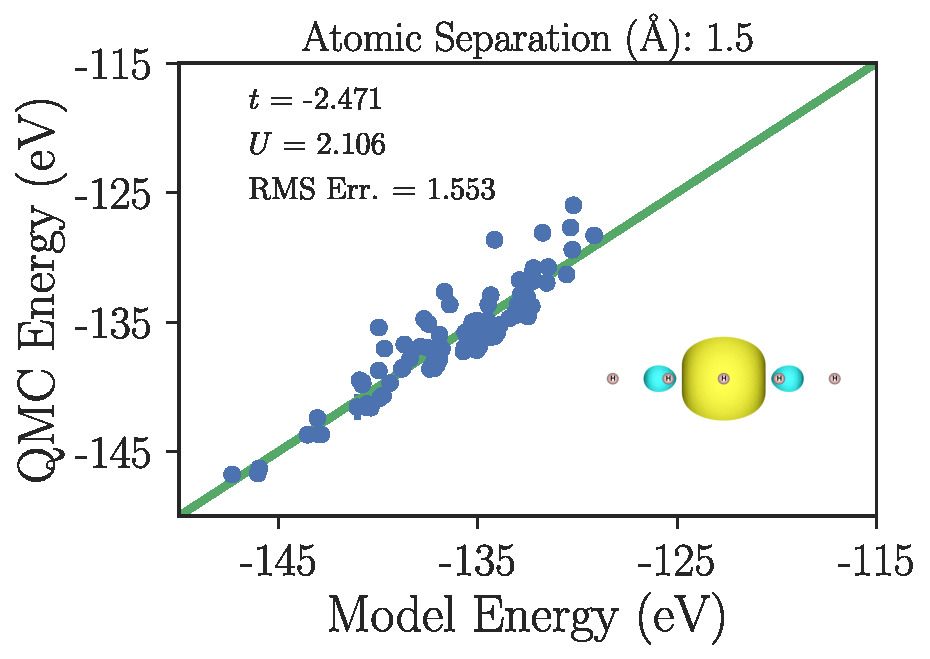
\includegraphics[scale=0.35]{{./Figures/H_chain_fit_model_length1.5_tUs_inset}.eps}
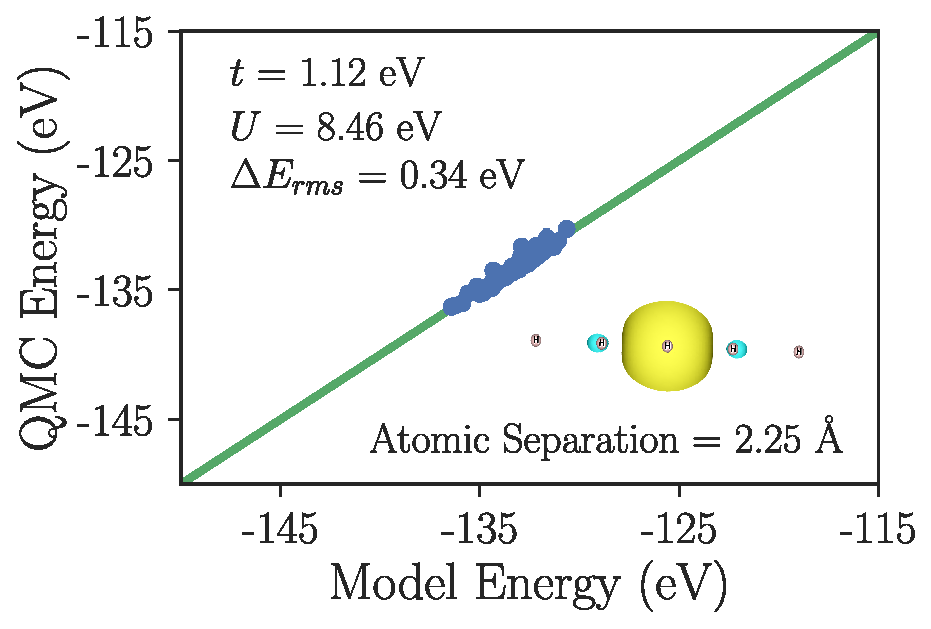
\includegraphics[scale=0.35]{{./Figures/H_chain_fit_model_length2.25_tUs_inset}.eps}
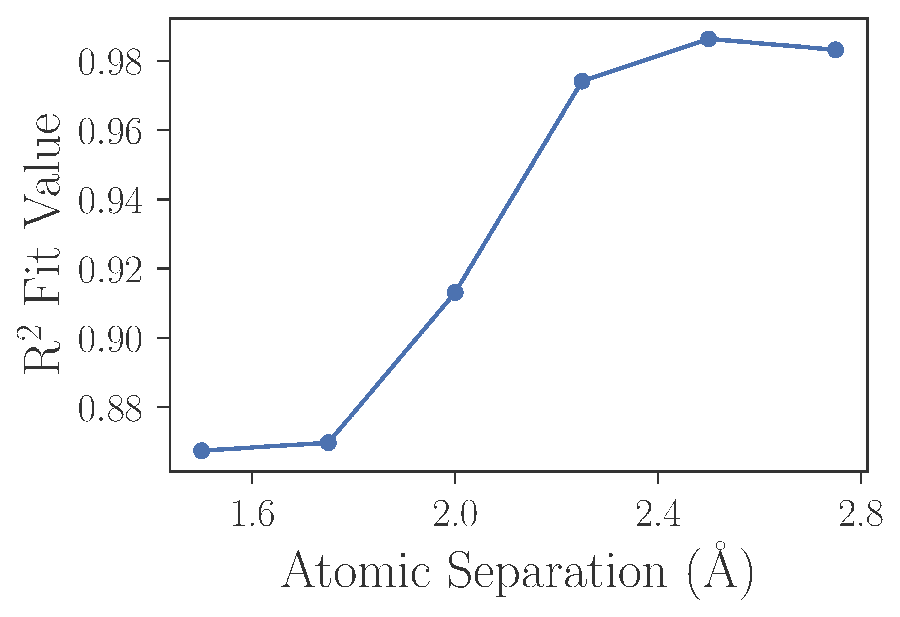
\includegraphics[scale=0.35]{{./Figures/r2_ut_vs_separation_h_chain}.eps}
\caption{Diffusion Monte Carlo energy versus the reconstructed 
model energy for the H$_{10}$ chain at (A) 1.5 \AA \: and (B) 2.25 \AA \:. The energy range of excitations 
narrows significantly for larger interatomic separation. Insets show the intrinsic atomic orbitals which constitute the one-body space 
which was used for calculating the reduced density matrices (descriptors). (C) The R$^2$ fit parameters obtained from fitting the $U$-$t$ model to the H$_{10}$ chain, as a function of interatomic separation.  
}
\label{fig:fit_quality}
\end{figure}

Fig.~\ref{fig:fit_quality} shows our DMD fits for two representative $r$. The model energy is the energy 
reconstructed from the optimized parameters $t$ and $U$ and the RDMs. For $r=1.5$ \AA \:, there is 
considerable spread in the data from the 45 degree line indicating that the simple short range Hubbard model 
is insufficient for an \textit{accurate} description in the corresponding energy window. In contrast, the R$^2$ fit parameter is significantly larger for larger $r$, suggesting the increased 
effectiveness of the one-band Hubbard model, as seen in Fig.~\ref{fig:fit_quality}(C). The insets show the intrinsic atomic orbitals for which we calculated 
the RDMs (descriptors). 

\begin{figure}
\centering
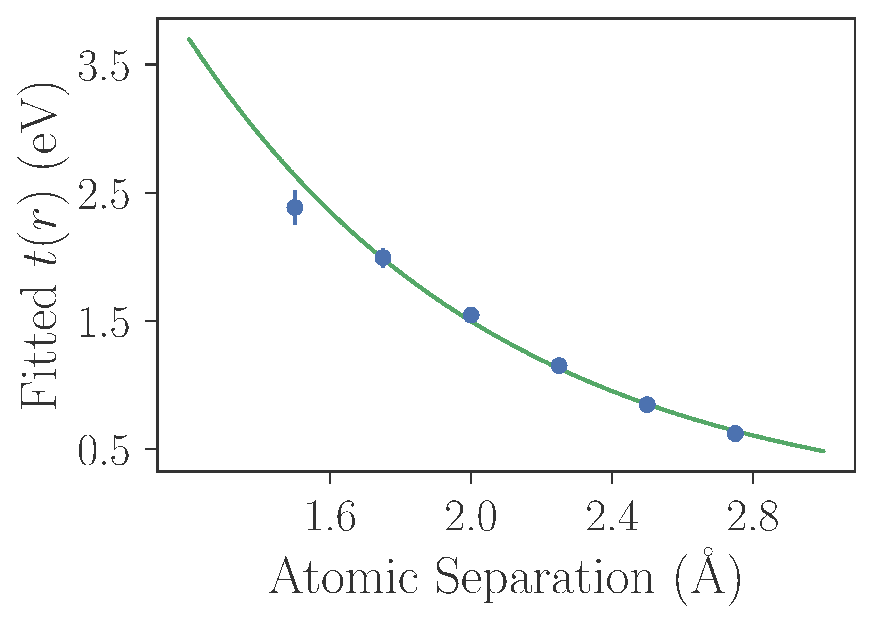
\includegraphics[scale=0.5]{./Figures/fitted_t_values_no_offset_h10_chain.eps}
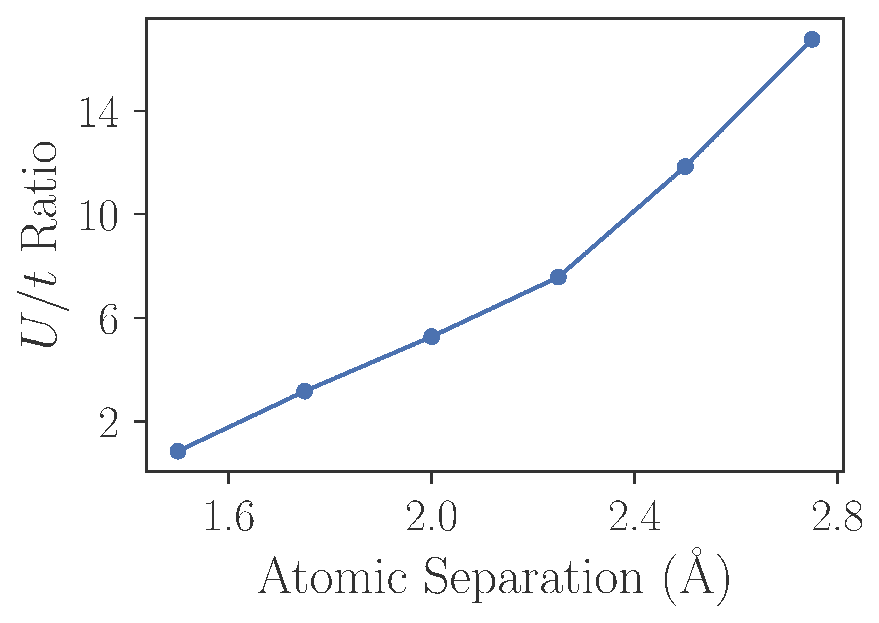
\includegraphics[scale=0.5]{./Figures/Ust_ratio_vs_separation_h_chain.eps}
\caption{(Left) The one-body hopping $t$ parameter as a function of interatomic distance for the periodic H$_{10}$ chain, obtained from a fitted $U$-$t$ model. $t$ declines to zero as $r$ increases. (Right) The ratio $U/t$ for the fitted parameter values as a function of interatomic separation. The ratio is small at lower bond-lengths, where $t$ is more relevant in describing the system, and larger at longer bond-lengths, where inter-site hopping is less significant. }\label{fig:Parameters-vs-Bond-t}
\end{figure}

Fig.~\ref{fig:Parameters-vs-Bond-t} shows trends of the DMD values of $t$ and $U$ as a function of $r$. 
Consistent with physical intuition, $t$ decreases towards zero at larger $r$
and the value of $U/t$ rises. However, as previously mentioned, the single-band 
Hubbard model is not expected to describe the hydrogen chain well at small distances. 
The one dimensional Hubbard model with $U/t>0$ will always result in 
an Mott insulating state. In comparison, for the idealized hydrogen chain, the 
metal-to-insulator transition has been shown to occur at $r_c \sim 1.8$\AA~\cite{Stella2011}, which would correspond 
to a finite non-zero $U$. This indicates that at small distance, the higher energy orbitals play a nontrivial 
role in stabilizing the metallic state of hydrogen, instead of merely renormalizing the effective strength of $U$. 
At small distances, other interactions like nearest neighbor Coulomb 
and exchange interactions also become important for $r<r_c$ \cite{ZhengThesis}. 

\subsection{Graphene and hydrogen honeycomb lattice}
\label{subsection:graphene}
Our third example highlights the role of the high energy 
degrees of freedom not present in the low energy description 
but which are instrumental in renormalizing the effective interactions. 
We demonstrate this by considering the case of graphene, and by 
comparing it to artificially constructed counterparts without the high energy electrons. 
Although many electronic properties of graphene can be adequately 
described by a noninteracting tight-binding model of $\pi$ electrons~\cite{Castro2009}, 
electron-electron interactions are crucial for explaining 
a wide range of phenomena observed in experiments~\cite{Kotov2012}. 
In particular, electron screening from $\sigma$ bonding renormalizes 
the low energy plasmon frequency of the $\pi$ electrons~\cite{Zheng2016}. In fact, 
without the $\sigma$ electrons, a system of $\pi$ electrons with bare Coulomb interactions has been shown \lucas{by whom? and why do we care that people argued it?} \HHZ{I changed the word "argue" to "shown". "by whom" is answered in the citations. We care the fact because it is directly related to our downfolding models. I added an extra sentence to strengthen this point} to be an 
insulator instead of a semimetal~\cite{DrutPRL2009, DrutPRB2009,  Smith2014, Zheng2016}. 
Using DMD, we demonstrate how the screening effect of $\sigma$ electrons is manifested in the low energy effective model of graphene. 

In order to disentangle the screening effect of $\sigma$ electrons from the bare interactions 
between $\pi$ electrons, we apply DMD to three different systems, graphene, $\pi$-only graphene, and a honeycomb lattice of hydrogen atoms.  
In the $\pi$-only graphene, the 
$\sigma$ electrons are replaced with a static constant negative charge background. 
The role of $\sigma$ electrons is then clarified by comparing the effective model Hamiltonians of these two systems. 
The hydrogen system we study has the same lattice constant $a=2.46$\AA~as graphene, 
which has a similar Dirac cone dispersion as graphene~\cite{Zheng2016}. 

By constructing the one-body space by Wannier localizing Kohn-Sham orbitals obtained from DFT calculations (see Fig.~\ref{fig:honeycomb_wan}), 
we verify that the low energy degrees of freedom correspond to the $\pi$ orbitals in graphene and 
its $\pi$-only system and $s$ orbitals in hydrogen; these enter the effective one-band Hubbard model description in Eq.~\eqref{eq:oneband}. 
Due to the vanishing density of states at the Fermi level, the Coulomb interaction remains long-ranged, 
in contrast to usual metals where the formation of electron-hole pairs screens the interactions strongly~\cite{Zheng2016}. 
However, for certain aspects, the long ranged part can be considered as renormalizing the 
onsite Coulomb interaction $U$ at low energy~\cite{Schuler2013, Changlani2015}. 
%Therefore, we expect that one-band Hubbard model is a reasonable description of the low energy physics. 
\lucas{Last sentence is not well-supported. In fact we know it has deficiencies and said so in our 2015 paper.}  \HHZ{I removed the last sentence.}
\renewcommand{\subfigimg}[3][,]{%
  \setbox1=\hbox{\includegraphics[#1]{#3}}% Store image in box
  \leavevmode\rlap{\usebox1}% Print image
  \rlap{\hspace*{20pt}\vspace*{18pt}\raisebox{\dimexpr\ht1-1.37\baselineskip}{#2}}% Print label
  \phantom{\usebox1}
}
\begin{figure}[hbt]
\centering
 \begin{tabular}{@{}p{0.90\linewidth}@{\quad}p{\linewidth}@{}}
   \subfigimg[clip, width=0.45\textwidth]{(A)}{./Figures/c_pi.eps}
   \subfigimg[clip, width=0.45\textwidth]{(B)}{./Figures/h_wan.eps}
 \end{tabular}
\caption{Wannier orbitals constructed from Kohn-Sham orbitals: (A) graphene $\pi$ orbital; (B) hydrogen $s$ orbital. \lucas{Need some kind of titles to differentiate the graphs. $E[\Psi]$ versus $E_{eff}[\Psi]$ }\HHZ{I assume you meant next figure.}}
\label{fig:honeycomb_wan}
\end{figure}

To estimate the one-band Hubbard parameters, we used the DMD method using a set of 50 Slater-Jastrow wave functions that correspond 
to the electron-hole excitations within the $\pi$ channel for the graphene systems 
or $s$ channel for the hydrogen system. In particular, for graphene, 
the Slater-Jastrow wave functions are constructed from occupied $\sigma$ bands and occupied $\pi$ bands, whereas for $\pi$-only 
graphene, Slater-Jastrow wave functions constructed from occupied $\pi$ Kohn-Sham orbitals of graphene. The \textit{ab initio} simulations 
were performed on a $3\times3$ cell (32 carbons or hydrogens) and the energy and RDMs of these wave functions were
evaluated with VMC. \footnote{We expect further renormalizations in the corresponding DMC calculations~\cite{Changlani2015}, 
but we do not explore that aspect here.\lucas{This is vague. Why should someone believe your results?} } The error bars on our downfolded parameters are estimated using the jackknife method.\lucas{citation} 
The results from our calculations are summarized in %Table~\ref{tab:grpheffm} 
Figure~\ref{fig:ne_aidmd_gh}.% shows the quality of the fits for the three systems.

%\begin{table}[ht]
%\centering
%\caption{Downfolding parameters for graphene and hydrogen.}
%\begin{tabular}{|c|c|c|c|}
%\hline
%Parameters [eV] & $\;\;\;\;$ graphene $\;\;\;$ & $\pi$-only graphene & $\;\;\;$hydrogen$\;\;\;$ \\
%\hline
%\hline
%$t$ & 3.61(1) & 2.99(1) & 3.73(1)\\
%$U$ & 7.16(3) & 14.8(2) & 9.47(5)\\
%\hline
%\end{tabular}

%\label{tab:grpheffm}
%\end{table} 
\renewcommand{\subfigimg}[3][,]{%
  \setbox1=\hbox{\includegraphics[#1]{#3}}% Store image in box
  \leavevmode\rlap{\usebox1}% Print image
  \rlap{\hspace*{42pt}\vspace*{12pt}\raisebox{\dimexpr\ht1-1.37\baselineskip}{#2}}% Print label
  \phantom{\usebox1}
}

\begin{figure}
\centering
  \begin{tabular}{@{}p{0.95\linewidth}@{\quad}p{\linewidth}@{}}
    \subfigimg[clip, width=0.325\linewidth]{(A)}{./Figures/grp_all_tu.eps}
    \subfigimg[clip, width=0.325\linewidth]{(B)}{./Figures/grp_pi_tu.eps}
    \subfigimg[clip, width=0.325\linewidth]{(C)}{./Figures/h_tu.eps}
    \end{tabular}
\caption{Comparison of \textit{ab initio} (x-axis) and fitted energies (y-axis) of the 3$\times$3 periodic unit cell of graphene and hydrogen lattice: (A) graphene; (B) $\pi$-only graphene; (C) hydrogen lattice.}\label{fig:ne_aidmd_gh}
\end{figure}

We find that the one-band Hubbard model describes graphene and hydrogen very well, as is seen from the fact that $R^2$ is closed to 1 for the fittings. \lucas{$R^2$ is a better supporter of this statement.} \HHZ{$R^2$ now is included in the plot.} of the predicted energies; our fits are shown in Figure~\ref{fig:ne_aidmd_gh}
For both graphene and hydrogen, $U/t$ is smaller than the critical value of the 
semimetal-insulator transition $(U/t)_c \approx 3.8$ for the honeycomb lattice~\cite{Sorella2012}, 
which is consistent with both systems being semimetals. The two systems indeed have similar hopping constant $t$, 
consistent with the fact that they have similar Fermi velocities at the Dirac point. However, 
the difference in their high energy structure manifests itself as different renormalizated electron-electrons interactions, 
explaining the difference in $U$. Most prominently, the $\pi$-only system has much larger $U/t$ ($\sim4.9$) compared to graphene, 
which is large enough to push it into the insulating (antiferromagnetic) phase. %of the honeycomb lattice Hubbard model. 
%Another important difference, which matches with our physical intuition,
\lucas{how so?} \HHZ{I deleted the statement about the hopping. That statement is not well supported quantitatively. } 
%is that graphene has larger $t$ than $\pi$-only graphene. 
%We attribute this to the $\sigma$ electrons pushing $\pi$ electrons away from the ions through exchange-correlation interactions, 
%which makes it easier for the $\pi$ electrons to hop to nearby sites. 
Thus, downfolding shows the clear significance of $\sigma$ electrons in renormalizing the effective onsite interactions of the $\pi$ orbitals,making graphene a weakly interacting semimetal instead of an insulator.  


%\subsection{FeSe diatomic molecule (NE-DMD)}
\subsection{FeSe diatomic molecule}
\label{subsection:fese}
\lucas{The basic problem we are trying to solve here is to choose parameterization. This needs to be up front.} 
Transition metal oxide systems are challenging to describe using most electronic structure methods because of the strong electron correlations and multiple oxidation states possible in these systems. %, and therefore, are an important test case for DMD. 
DMC has been shown to be a highly accurate method on transition metal oxide materials, where it has been shown to improve the description of the ground state properties and energy gaps~\cite{Foyevtsova2014, Wagner_Abbamonte, Zheng2015, Wagner2016}. % for the types of orbital excitations used to sample the Hilbert space.
However, given the expense of large DMC calculations, finding effective models consistent with DMC would be valuable for studying extended transition metal oxide systems at large scale.
Additionally, these complex systems usually involve competing interactions that give rise to novel phenomena. 
DMD could help\lucas{could help? vague} to identify important physics degrees of freedom relevant to macroscopic phenomena.
In particular, utilizing matching pursuit \lucas{we haven't explained matching pursuit} and DMD to find minimal descriptions could offer a way to quantify the relative importance of different interactions.

As a test\lucas{what are we testing? I didn't see any test.} of DMD for transition metal oxide systems, we consider an FeSe diatomic molecule with atomic separation 2.43 \AA~in the $z$-direction.
To our knowledge, this FeSe diatom does not exist in nature, but nevertheless serves as a simple illustration of a model for the interaction between a transition metal and a ligand. 
The bond distance is chosen to match the unconventional superconductor, FeSe~\cite{kumar_crystal_2010}, and therefore offer insight into a model description for FeSe solid in future studies.

\lucas{This paragraph is trying to do too many things. It needs to be separated. One paragraph for generation of low energy states, one for the model parameterization, one for the MP method, maybe another?}
We consider a model including one iron $4s$, five iron $3d$ states, and three selenium $4p$ states:
\begin{align}
  H 
  &=
  \epsilon_{xy} \sum_{\eta} (n^{d_{xy}}_{\eta}  + n^{d_{x^2-y^2}}_{\eta})
  +
  \epsilon_s \sum_{\eta} n^{s}_{\eta} 
  +
  \epsilon_{p_{z}} \sum_{i,\eta} n^{p_{z}}_{i,\eta} 
  \nonumber \\
  &+ 
  t_{\sigma,d} \sum_{\eta} \left( d_{z^2,\eta}^{\dagger} p_{z,\eta} + \text{h.c.} \right)
  +
  t_{\sigma,s} \sum_{\eta} \left(s_{\eta}^{\dagger}  p_{z,\eta} + \text{h.c.} \right)
  \nonumber \\
  &+
  U_d \sum_{i} n^{d}_{i,\uparrow} n^{d}_{i,\downarrow} 
  +
  J_d \sum_{i\ne j} S_i \cdot S_j
  +
  E_0. \label{eq:fesemodel}
\end{align}
\lucas{clarify notation. There are some orbitals in superscripts. some in subscripts. Should be $\hat{n}'s$. }
Here, $\eta$ is the spin index and $i$ is the orbital index.
The $\epsilon_i$'s are single-particle orbital energies, while the $U_d$ is an on-site interaction among the $d$ orbitals and the $J_d$ is a Hund's coupling among the $d$ orbitals.
$E_0$ is an overall energy shift.
This set of parameters was chosen based on the matching pursuit method described in Sec.~\ref{sec:theory}.
\lucas{It was not described there.}
The MP was able to choose from a set of 21 symmetry allowed $\epsilon$, $t$, $U$, and $J$ parameters as it included parameters.  \lucas{List the parameters that we chose from.}
For this demonstration, we add parameters one at a time until the RMS error drops by less than 0.05 eV. 
\lucas{Why did we stop there? There are much better ways like I mentioned before like test/training, even something like BIC is better.} 
With this criteria, the 8 parameters in Eq.~\ref{eq:fesemodel} are included, the final RMS error is 0.61 eV, the final coefficient of determination ($R^2$) is 0.84, and the next parameter in the algorithm increases the $R^2$ by less than 0.02. \lucas{We are switching between RMS and R$^2$}
For example, $U_p$, an on-site interaction for the Se $p$-electrons, does not correlate strongly enough\lucas{strongly enough is vague} with the residuals, and is not included before the algorithm halts.
The states sampled consisted of singles and doubles excitations from PBE0 calculations with total spin 0, 2, and 4, which were then relaxed via a DMC projection.
233 states fit within an energy window of 8 eV from the ground state, and were selected as the low energy space.
Eight states within the window are not considered because the sum of all occupation descriptors was more than 0.5 less than the number of electrons.
These states generally\lucas{generally is vague.} have a significant iron $4p$ component relative to the ground state, and therefore were excluded, since they are not describable without several additional parameters describing the iron $p$ states. \lucas{why are we ok excluding them?}

\begin{figure*}
  \centering
  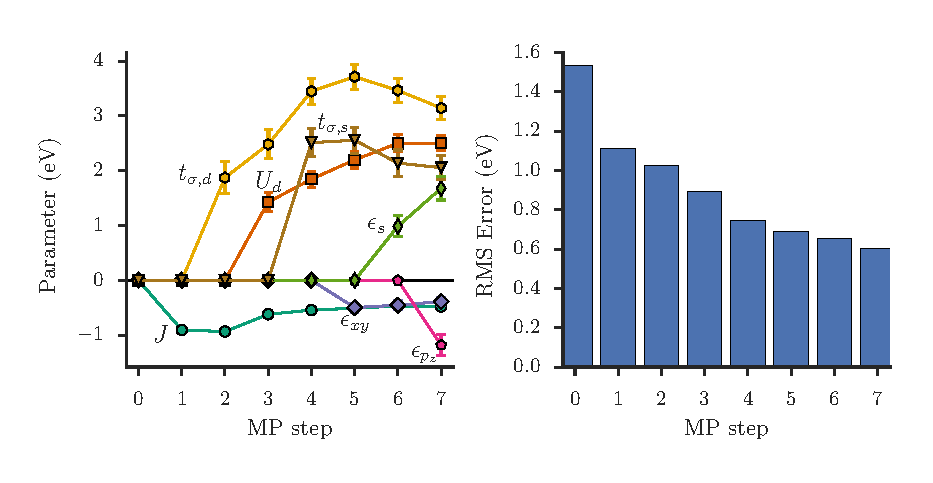
\includegraphics[width=0.8\textwidth]{./Figures/fese.eps}
  \caption{
    \label{fig:fese} 
    (A) Parameter values for each fit generated in the MP algorithm, labeled at the step where they are included in the model. 
    A zero value indicates that parameter is not yet added to the model.
    The sign of $J$ is consistent with Hund's rules, and the signs of $t_{\sigma,d}$ and $t_{\sigma,s}$ are consistent with Se being located in positive $z$ with respect to Fe. 
    The $\epsilon_i$ states adjust the energies of the single particle orbitals relative to the energy of the other orbitals.
    (B) RMS error of each model generated by MP as the algorithm includes parameters. 
  }
\end{figure*}

Applying the MP approach to the system produced reasonable parameter estimates, and suggested the Hund's coupling to be an important component of this model.
\lucas{too much passive, 'reasonable,' 'suggested'}
Figure~\ref{fig:fese}(a) and (b) show the evolution of the parameters and RMS error of the fit parameters are added one by one.
All previous parameters may change at each step because the entire model is refitted in each iteration.
The parameters are smoothly varying with the inclusion of new parameters, and their values are physically reasonable.
The matching pursuit algorithm would suggest that minimal models can be built by disregarding the descriptors added in later steps.
For this system, $J$ is considered the most important parameter\lucas{'most important' is vague. Don't use that construction.} in the model, and an absolute minimal model for the system would be $H_\text{minimal} = E_0 + J_d \sum_i S_i \cdot S_j$. 
Such a model would have an RMS error 1.11 eV. 
According to matching pursuit, the next most important interactions to include are (1) hopping between $d_{z^2}$ and $p_z$, (2) on-site $d$ Coulomb interactions, and (3) hopping between the $4s$ and the $p_z$, and so on. 
Including these degrees of freedom brings the RMS error to 0.75 eV.\lucas{What does this mean?} 
In this way, MP would suggest\lucas{MP doesn't suggest anything. Things don't suggest.}  that the most important interactions in the system at low energy are Hund's coupling, hopping between iron $3d$ and selenium $4p$, and on-site Coulomb repulsion, in that order.
This observation is consistent with the several studies in the literature, which find Hund's coupling in bulk FeSe to be an important part of its description~\cite{demedici_hunds_2011,de_medici_janus-faced_2011,georges_strong_2013,busemeyer_competing_2016}.


\section{Conclusion and Future prospects}
To summarize, we have explained the AIDMD method that we have been developing, primarily in conjunction with the 
\emph{ab-initio} QMC approach. The practical motivation is to take data from first principles (continuum) 
calculations as inputs for lattice model (discrete) methods. 
Since one is mapping a many body problem to a few body one, the relevant quantities of interest are 
the reduced density matrices associated with the many-body wavefunctions projected to a one-body space. 
The density matrix based approach is appealing as it is democratic 
in the determination of the hopping and interaction parts of the effective Hamiltonian, and provides multiple 
checks on its validity. We have discussed representative examples to present the conceptual and algorithmic aspects of AIDMD. 

What sort of accuracy should one expect with effective Hamiltonians and AIDMD? The holy grail of quantum chemistry 
and electronic structure is to obtain an energy of 1 mHa (0.027 eV) per atom; this 
remains an open challenge despite decades of work. The effective Hamiltonian approach somewhat ameliorates 
this problem, only relative energies are important, neither the total energy (nor its accuracy) is of particularly 
fundamental interest. This is contingent on the cancellation of the large energy associated with the core electrons, 
whose role is to primarily renormalize the interactions between the active (valence) electrons. This aspect can also 
be a major limitation when the core and active electrons are strongly entangled i.e when the separation of energy 
scales is not prominent (in which case an energy-dependent description may be needed). 
Thus, it is possibly best suited for extended systems (solids) where this separation exists. 
In our view, AIDMD (and downfolding in general) opens up many avenues for determination of physical 
quantities not easily calculated in ground state approaches. Our experience suggests excitation spectra 
can be accurately determined to 0.2 eV (or less)~\cite{Changlani2015} and potentially improved with 
more \emph{ab-initio} data and more refined effective Hamiltonians.  

Finally we would like to emphasize that AIDMD, though conceptually simple, 
is still a method in its development stages, with room for algorithmic improvements and new applications. It suffers 
from the usual problems of optimization and overfitting, but with advances in these fields we believe some of these major 
concerns may become less problematic. Some of the issues that need further research are,
\begin{itemize} 
	\item Construction of wavefunction database:
	The AIDMD method relies crucially on the availability of a low energy space of \emph{ab initio} wavefunctions, 
	which despite not being eigenstates, reveal the nature of the effective Hamiltonian. Automating its construction 
	remains somewhat challenging. We propose Slater Jastrow wavefunctions and deforming the orbitals entering the Slater 
	determinant as one way of probing the low energy manifold.
	\item Optimal choice of active orbitals (one body space):
	In the present work, we chose DFT orbitals (in a certain energy window) and localized them to get the one body orbitals. 
	The choice could only be justified based on looking at the trace of the 1-RDM and ensuring that it 
	equalled the expected number of electrons. We expect to use intrinisic atomic orbitals (pointed out to us by G. K. Chan) which 
	mitigate this issue. 
	\item Form of the low energy model Hamiltonian:
	Extensive work in the literature has been devoted to parameterizing compact effective Hamiltonians~\cite{Georges, Oles, Coury}. 
	Since the low energy effective Hamiltonian is not unique, there is not necessarily one right way of downfolding. 
	One could catalogue all functional forms based on previous parameterizations 
	or there may be some merit in determining the minimal description with fewest non zero parameters.
	Note that most models for strong correlation \emph{assume} two body forms. While this appears to work well in practice, 
	it is by not guaranteed on mathematical grounds. (Even though the Coulomb operator is two body, 
	its low energy description need not be.) In this regard, AIDMD could also be used to assess 
	the accuracy of DFT based downfolding methods.
	\item Other (non QMC) wavefunction based electronic structure methods:
	There are several wavefunction based quantum chemistry 
	methods for electronic structure like coupled cluster and ab-initio DMRG which work primarily 
	directly in orbital space. These could also be potentially explored in conjunction with AIDMD.
\end{itemize} 

In terms of applications, we hope the method will be eventually applied to solids involving transition 
metals and/or rare earth elements, which are in the strongly correlated regime due to the presence of localized orbitals. 
Some challenging areas include,
\begin{itemize} 
	\item Spin models for magnetism: 
	The magnetism associated with strongly correlated Mott insulators, compounded by effects such as geometrical frustration, 
	is highly non trivial and has become an active area of research in its own right. 
	%This is compounded by 
	%the presence of geometric frustration, impurities and defects and 
	%spin-orbital effects. 
	For example, the two dimensional kagome lattice planes in 
	herbertsmithite harbor an exotic topological phase of matter - a "quantum spin liquid". While our understanding is primarily 
	from Heisenberg models~\cite{Yan_Huse_White, Changlani_kagome}, 
	contentious issues plague a complete understanding and connection to experiment (there has been recent progress 
	in downfolding herbertsmithite~\cite{Jeschke}). 
	Other areas of application include pyrochlore iridates and titanates and Kitaev materials. 
	We caution that relevant energy scales associated with magnetism can be $0.1$ meV or less, and no electronic structure 
	method is currently that accurate. It may thus be necessary to perform multiple downfolding steps to map from 
	the Schrodinger equation to a spin model.
	\item Multiband models for superconductors:
	As previously mentioned, unconventional (non BCS) superconductivity in materials such as the cuprates and iron based 
	pntictides has fuelled the study of strongly correlated systems.
	Several parameter sets exist in the literature for multi-band models, but it appears that there is little universal consensus. 
	We are optimistic that additional \emph{ab-initio} inputs from AIDMD will help constrain the part of parameter 
	space relevant for these materials. Trends of the parameters (and the effectiveness of the three band 
	or one band model itself) with pressure dependence and doping remain largely unexplored.  
	%\item Quantum computing (\HJC{tell me if this one is too weird}) : 
	%Quantum computers have been heralded as the future of computing with many promising advances. 
	%There has been progress in the simulation of small molecules in compact basis sets, but scalability (needed for solids) 
	%remains an issue. Downfolding macould help in the reduction in the number of active orbitals 
\end{itemize} 

\section{Acknowledgements} 
We thank  David Ceperley,  Richard Martin, Cyrus Umrigar,  Garnet Chan,  Shiwei Zhang, Steven White,  
Lubos Mitas, So Hirata, Bryan Clark, Norm Tubman, Miles Stoudenmire and Victor Chua for extremely useful and insightful discussions. 
This work was funded by the grant DOE FG02-12ER46875 (SciDAC). HJC acknowledges support from the U.S. Department of Energy, 
Office of Basic Energy Sciences, Division of Materials Sciences and Engineering under Award DE-FG02-08ER46544 for his work at the Institute for Quantum Matter (IQM). 

\section*{Author Contributions}
HJC, HZ and LKW conceived the initial DMD ideas and designed the project and organization of the paper. 
All authors contributed to the theoretical developments and various representative \textit{ab-initio} and lattice examples. 
All authors contributed to the analysis of the data, discussions and writing of the manuscript. 
LKW oversaw the project. HJC and HZ contributed equally to this work.
 
\section*{Additional Information}
Competing financial interests: The authors declare no competing financial interests.


%\bibliographystyle{unsrt}
\bibliographystyle{frontiersinHLTH&FPHY} 
\bibliography{refs}

\end{document}
